%% Copernicus Publications Manuscript Preparation Template for LaTeX Submissions
%% ---------------------------------
%% This template should be used for copernicus.cls
%% The class file and some style files are bundled in the Copernicus Latex Package which can be downloaded from the different journal webpages.
%% For further assistance please contact the Copernicus Publications at: publications@copernicus.org
%% http://publications.copernicus.org


%% Please use the following documentclass and Journal Abbreviations for Discussion Papers and Final Revised Papers.


%% 2-Column Papers and Discussion Papers
\documentclass[gmd, manuscript]{copernicus}



%% Journal Abbreviations (Please use the same for Discussion Papers and Final Revised Papers)

% Archives Animal Breeding (aab)
% Atmospheric Chemistry and Physics (acp)
% Advances in Geosciences (adgeo)
% Advances in Statistical Climatology, Meteorology and Oceanography (ascmo)
% Annales Geophysicae (angeo)
% ASTRA Proceedings (ap)
% Atmospheric Measurement Techniques (amt)
% Advances in Radio Science (ars)
% Advances in Science and Research (asr)
% Biogeosciences (bg)
% Climate of the Past (cp)
% Drinking Water Engineering and Science (dwes)
% Earth System Dynamics (esd)
% Earth Surface Dynamics (esurf)
% Earth System Science Data (essd)
% Fossil Record (fr)
% Geographica Helvetica (gh)
% Geoscientific Instrumentation, Methods and Data Systems (gi)
% Geoscientific Model Development (gmd)
% Geothermal Energy Science (gtes)
% Hydrology and Earth System Sciences (hess)
% History of Geo- and Space Sciences (hgss)
% Journal of Sensors and Sensor Systems (jsss)
% Mechanical Sciences (ms)
% Natural Hazards and Earth System Sciences (nhess)
% Nonlinear Processes in Geophysics (npg)
% Ocean Science (os)
% Proceedings of the International Association of Hydrological Sciences (piahs)
% Primate Biology (pb)
% Scientific Drilling (sd)
% SOIL (soil)
% Solid Earth (se)
% The Cryosphere (tc)
% Web Ecology (we)
% Wind Energy Science (wes)


%% \usepackage commands included in the copernicus.cls:
%\usepackage[german, english]{babel}
%\usepackage{tabularx}
%\usepackage{cancel}
%\usepackage{multirow}
%\usepackage{supertabular}
%\usepackage{algorithmic}
%\usepackage{algorithm}
%\usepackage{amsthm}
%\usepackage{float}
%\usepackage{subfig}
%\usepackage{rotating}

\usepackage{subcaption}

% Custom commands
\newcommand{\vb}{\mathbf}
\newcommand{\vg}{\boldsymbol}
\newcommand{\mat}{\mathsf}
\newcommand{\diff}[2]{\frac{d #1}{d #2}}
\newcommand{\diffsq}[2]{\frac{d^2 #1}{{d #2}^2}}
\newcommand{\pdiff}[2]{\frac{\partial #1}{\partial #2}}
\newcommand{\pdiffsq}[2]{\frac{\partial^2 #1}{{\partial #2}^2}}

% User-defined mathematical symbols
\renewcommand{\emph}[1]{{\color{red}\textbf{#1}}}
\newcommand{\pd}[2]{\frac{\partial #1}{\partial #2}}
\newcommand{\p}[1]{\partial #1}
%Then, writing a partial is as simple as $\pd{J}{x}$.
\newcommand{\ol}[1]{{\overline #1}}
\newcommand{\mbf}[1]{{\mathbf #1}}
\newcommand{\mbfol}[1]{\overline{{\mathbf #1}}}
\newcommand{\wdh}[1]{{\widehat #1}}
\newcommand{\wdt}[1]{{\widetilde #1}}
\newcommand{\sss}[1]{{\scriptscriptstyle #1}}
\newcommand{\scs}[1]{{\scriptstyle #1}}


\begin{document}

\title{DCMIP2016, Part 1: Models and Equation Sets}


% \Author[affil]{given_name}{surname}

\Author[1]{Paul A.}{Ullrich}
\Author[2]{Christiane}{Jablonowski}
\Author[3]{James}{Kent}
\Author[4]{Peter H.}{Lauritzen}
\Author[4]{Ramachandran}{Nair}
\Author[5]{Kevin A.}{Reed}
\Author[4]{Colin M.}{Zarzycki}

\Author[6]{David A.}{Hall}

\Author[7]{Alex}{Reinecke}
\Author[7]{Kevin}{Viner}

\Author[8]{Don}{Dazlich}
\Author[8]{Ross}{Heikes}
\Author[8]{Celal}{Konor}
\Author[8]{David}{Randall}

\Author[9]{Xi}{Chen}
\Author[9]{Lucas}{Harris}

\Author[10]{Marco}{Giorgetta}
\Author[11]{Daniel}{Reinert}

\Author[12]{Christian}{Kuehnlein}

\Author[13]{Robert}{Walko}

\Author[14]{Vivian}{Lee}
\Author[14]{Abdessamad}{Qaddouri}
\Author[14]{Claude}{Girard}

\Author[15]{Hiroaki}{Miura}
\Author[15]{Tomoki}{Ohno}
\Author[16]{Ryuji}{Yoshida}

\Author[4]{Joseph}{Klemp}
\Author[4]{Sang-Hun}{Park}
\Author[4]{William}{Skamarock}

\Author[17]{Thomas}{Dubos}
\Author[17]{Yann}{Meurdesoif}

\Author[18]{Elijah}{Goodfriend}
\Author[18]{Hans}{Johansen}

\affil[1]{University of California, Davis}
\affil[2]{University of Michigan}
\affil[3]{University of South Wales}
\affil[4]{National Center for Atmospheric Research}
\affil[5]{Stony Brook University}
\affil[6]{University of Colorado, Boulder}
\affil[7]{Naval Research Laboratory}
\affil[8]{Colorado State University}
\affil[9]{Geophysical Fluid Dynamics Laboratory}
\affil[10]{Max Planck Institute for Meteorology}
\affil[11]{Deutscher Wetterdienst (DWD)}
\affil[12]{European Center for Medium-Range Weather Forecasting}
\affil[13]{University of Miami}
\affil[14]{Environment Canada}
\affil[15]{University of Tokyo}
\affil[16]{RIKEN}
\affil[17]{Institut Pierre-Simon Laplace (IPSL)}
\affil[18]{Lawrence Berkeley National Laboratory}

%% The [] brackets identify the author with the corresponding affiliation. 1, 2, 3, etc. should be inserted.



\runningtitle{DCMIP2016: Models and Equation Sets}

\runningauthor{Ullrich, et al.}

\correspondence{Paul A. Ullrich (paullrich@ucdavis.edu)}



\received{}
\pubdiscuss{} %% only important for two-stage journals
\revised{}
\accepted{}
\published{}

%% These dates will be inserted by Copernicus Publications during the typesetting process.


\firstpage{1}

\maketitle



\begin{abstract}
This paper provides a comprehensive review of the design of modern non-hydrostatic atmospheric dynamical cores, including relevant equation sets, numerical stabilization techniques and idealized physics routines.
\end{abstract}



\introduction  %% \introduction[modified heading if necessary]

{\color{red}INSTRUCTIONS FOR AUTHORS: Fill in text in section 3, 4, 5, 6, 7 and 8 below.}

The Dynamical Core Model Intercomparison Project (DCMIP) is an ongoing effort targeting the intercomparison of a fundamental component of global atmospheric modeling systems: the dynamical core.  Although this component's role is simply to solve the equations of fluid motion (the Navi\'er-Stokes equations) throughout the atmosphere, there are numerous confounding factors that arise as a consequence of compromises that are required to make simulation computationally feasible.  These factors include the choice of model grid, vertical coordinates, representation of topography, numerical method, physics/dynamics coupler, and the manner in which artificial diffusion, filters and/or energy/mass fixers are applied.

To advance the intercomparison project and provide a unique educational opportunity for students, DCMIP has hosted a multidisciplinary two-week summer school and model intercomparison project, held at the National Center for Atmospheric Research (NCAR) in June 2016, that invited graduate students, postdocs, atmospheric modelers, expert lecturers and computer specialists to create a stimulating, unique and hands-on driven learning environment. It was built on previous intercomparison efforts by addressing key outstanding issues in global atmospheric models, incorporate international participation, and provide a unique training experience for the future generation of climate scientists. Special attention is paid to the role of simplified physical parameterizations, physics-dynamics coupling, non-hydrostatic atmospheric modeling and variable-resolution global modeling. The summer school and model intercomparison project promoted active learning, innovation, discovery, mentorship and the integration of science and education.

The summer school directly benefited its participants by providing a unique educational experience and an opportunity to interact with modeling teams from around the world.  The workshop is expected to have further repercussions on the development of operational atmospheric modeling systems, by giving modeling groups an opportunity to assess and intercompare their models with other advanced modeling systems.  Modeling groups have already begun to leverage this information to improve their own models, which will in turn positively impact the quality of weather and climate simulations going forward.

The proposed workshop has advanced our knowledge of (a) the relative behaviors exhibited by atmospheric dynamical cores, (b) differences that arise among mechanisms for coupling the physical parameterizations and dynamical core, and (c) the impacts of variable-resolution refinement regions and transition zones in global atmospheric simulations.  Notably, the use of idealized test cases isolating specific phenomena gave us a unique opportunity to assess specific differences that arise due to the choice of dynamical core.  A key outcome of the workshop was the development of a standard test case suite and benchmark set of simulations that can be used for assessment of any future dynamical core.

\section{Notation}

\subsection{List of Symbols}

Table \ref{tab:symbols} lists the symbols used in this paper.

\begin{table}[h]
\caption{List of symbols used in this manuscript} \label{tab:symbols}
\begin{center}
\begin{tabular}{cl}
\hline Symbol & Description \\ \hline 
$\lambda$ & Longitude (in radians) \\
$\varphi$ & Latitude (in radians) \\
$z$ & Height with respect to mean sea level (set to zero) \\
$p_s$ & Surface pressure ($p_s$ of moist air if $q>0$) \\
$\Phi_s$ & Surface geopotential \\
$z_s$ & Surface elevation with respect to mean sea level (set to zero) \\
$u$ & Zonal wind \\
$v$ & Meridional wind \\
$w$ & Vertical velocity \\
$\omega$ & Vertical pressure velocity  \\
$\delta$ & Divergence\\
$\zeta$ & Relative vorticity\\
$p$ & Pressure (pressure of moist air if $q>0$) \\
$\rho$ & Total air density \\
$\rho_d$ & Dry air density \\
$T$ &Temperature \\
$T_v$ & Virtual temperature \\
$\Theta$ & Potential temperature \\
$\Theta_v$ & Virtual potential temperature \\
$q$ & Specific humidity \\
$P_{ls}$ & Large-scale precipitation rate \\
$q_c$ & Cloud water mixing ratio \\
$q_r$ & Rain water mixing ratio \\
\hline 
\end{tabular}
\end{center}
\end{table}

\subsection{List of Physical Constants}
A list of physical constants which are used throughout this document is given in Table \ref{tab:PhysicalConstants}.  Constants which are specific to each test case are similarly tabulated at the beginning of each section.

\begin{table}[h]
\caption{A list of physical constants used in this document.} \label{tab:PhysicalConstants}
%\ \\
\begin{tabular*}{\textwidth}{@{\extracolsep{\fill}}lll}
\hline Constant & Description & Value \\
\hline $a_{\tiny \mbox{ref}}$ & Radius of the Earth & $6.37122 \times 10^{6}\ \mbox{m}$ \\
$\Omega_{\tiny \mbox{ref}}$ & Rotational speed of the Earth & $7.292\ \times 10^{-5}\ \mbox{s}^{-1}$ \\
%$a$ & Scaled radius of the Earth & $a_{\tiny \mbox{ref}} / X$ \\
%$\Omega$ & Scaled rotational speed of the Earth & $\Omega_{\tiny \mbox{ref}} \cdot X$ \\
$g_c$ & Gravitational acceleration & $9.80616\ \mbox{m}\ \mbox{s}^{-2}$ \\
$p_0$ & Reference pressure & $1000\ \mbox{hPa}$ \\
$c_{pd}$ & Specific heat capacity of dry air at constant pressure & $1004.5\ \mbox{J}\ \mbox{kg}^{-1}\ \mbox{K}^{-1}$ \\
$c_{pw}$ & Specific heat capacity of water vapor at constant pressure & $1930.0\ \mbox{J}\ \mbox{kg}^{-1}\ \mbox{K}^{-1}$ \\
$c_{vd}$ & Specific heat capacity of dry air at constant volume & $717.5\ \mbox{J}\ \mbox{kg}^{-1}\ \mbox{K}^{-1}$ \\
$c_{vw}$ & Specific heat capacity of water vapor at constant volume & $1460.0\ \mbox{J}\ \mbox{kg}^{-1}\ \mbox{K}^{-1}$ \\
$R_d$ & Gas constant for dry air & $287.0\ \mbox{J}\ \mbox{kg}^{-1}\ \mbox{K}^{-1}$ \\
$R_w$ & Gas constant for water vapor & $461.5$ J kg$^{-1}$ K$^{-1}$ \\
%$\kappa$ & Ratio of $R_d$ to $c_p$ & $2/7$ \\
$\varepsilon$ & Ratio of $R_d$ to $R_w$ & $0.622$ \\
$M_v$ & Constant for virtual temperature conversion & $0.608$ \\
$\rho_{water}$ & Reference density of water & 1000 kg m$^{-3}$ \\
\hline 
\end{tabular*}

\end{table}

\subsection{Great Circle Distance}

The great circle distance is used throughout the document and is given by
\begin{equation}
R_c(\lambda_1, \varphi_1; \lambda_2, \varphi_2) = a \arccos \left( \sin \varphi_1 \sin \varphi_2 + \cos \varphi_1 \cos \varphi_2 \cos (\lambda_1 - \lambda_2) \right).
\end{equation}

%%%%%%%%%%%%%%%%%%%%%%%%%%%%%%%%%%%%%%%%%%%%%%%%%%%%%%%%%%%%%

\section{Model Grids} \label{sec:ModelGrids}

\subsection{Latitude-longitude grid}

The classic latitude-longitude grid consists of a subdivision of the sphere produced by subdividing along lines of constant latitude and longitude {\color{red}[Figure]}.  Because of the convergence of grid lines near the poles, the operational use of this grid requires that the associated numerical scheme be resilient to arbitrarily small Courant number, or that polar filtering be employed to remove unstable computational modes \citep{lin2004vertically}.  This grid is employed by the UK Met Office \citep{davies2005new}.

\subsection{Cubed-sphere grid}

The equiangular gnomonic cubed-sphere grid \citep{sadourny1972conservative, ronchi1996cubed} consists of six Cartesian patches arranged along the faces of a cube which is then inflated onto a spherical shell.  More information on this choice of grid can be found in \cite{ullrich2014global}.  On the equiangular cubed-sphere grid, coordinates are given as $(\alpha, \beta, p)$, with central angles $\alpha, \beta \in [- \frac{\pi}{4}, \frac{\pi}{4}]$ and panel index $p$.  The structure of this grid supports refinement through stretching \citep{Schmidt1977,harris2016high} or nesting \citep{harris2013two}.  The Cartesian structure of cubed-sphere grid panels is advantageous for numerical methods that are formulated in Cartesian coordinates, or that utilize dimension splitting.  Nonetheless, special treatment of the panel boundaries is often necessary since they represent coordinate discontinuities. {\color{red}[Cubed-sphere grid figure]}

%FV$^3$ is discretized on the equiangular gnomonic cubed-sphere grid as described in \citet{PL2007JCP}. The gnomonic cubed sphere was found to yield the best balance of uniformity and simplicity for use with the FV algorithm. The structure of this grid supports refinement through stretching \citep{Schmidt1977,harris2016high} or nesting \citep{harris2013two}.  The convention for panel numbering used in FV$^3$ differs from that described above, so that odd-numbered panels are adjacent to the next-higher-numbered panel on their right-hand side, and even-numbered panels are adjacent to the next-higher numbered panel on their top side. 

\subsection{Icosahedral (triangular) grid}

For the common global applications, the icosahedral triangular grid is derived from the spherical icosahedron that consists of 20 equilateral spherical triangles, 30 great circle edges and 12 vertices.  These initial triangles are then subdivided repeatedly until the desired mean resolution is obtained. For a single subdivision each edge is divided in $n$ arcs of equal length, thus defining new vertices, which by proper connection to other new vertices result in $n^{2}$ triangles filling the original triangle. By construction the new vertices share 6 triangles, thus the refinement process brakes the initial isotropy of the icosahedron and results in non-equilateral triangles of different sizes.

Several methods are available for subdividing the triangular regions.  One such approach is implemented by the ICON grid generator, which allows an ``arbitrary'' subdivision factor $n$ for the first refinement step only, the so-called root refinement. Typical choices are $n$ = 2, 3 or 5. All additional $m$ refinement steps use $n$ = 2, i.e. are bisection steps. A global grid resulting from a root division factor $n$ and $m$ bisections, denominated as \textit{RnBm} grid,  has $n_c = 20 \cdot n^2 \cdot 2^{2m}$ cells, $n_e = 3/2 \cdot n_c$ edges and $n_v = 10\cdot n^{2}\cdot 2^{2m}+2$ vertices. The anisotropy of global grids is reduced by the spring dynamics of \cite{tomita2001}.  For a discussion of the effective resolution see \cite{dipankar2015large}.  The ICON grid generator further allows for inset regional grids, produced by additional refinement steps that are only applied over a limited region, or set of regions.  The dynamical core then allows for either one-way or two-way coupling of the refined region to the parent model. The current operational numerical weather prediction of the Deutscher Wetterdienst (German Weather Service, DWD) for instance uses a $R3B7$ global grid with 2949120 cells and 13 km mean resolution in combination with a refined region over Europe at 6.5 km resolution.

\subsection{Icosahedral (hexagonal) grid}

\subsection{Constrained Centroidal Voronoi Tessellation (CCVT) grids}

Given a set of $N$ distinct points on the sphere $x_i$ (referred to as the generators, $1 \leq i \leq N$), the \textit{Voronoi tessellation} (or the \textit{Voronoi diagram}) associated with the generators is the set of polygons $\Omega_i$ consisting of all points that are closer (in the sense of great-circle distance) to $x_i$ than any other $x_j$ with $i \neq j$ \citep{okabe2009spatial}.  For a given set of generators, this tiling is unique and completely covers the sphere, and so can be employed in conjunction with many finite volume methods.  However, for an arbitrary set of generators it is easy to produce highly distorted polygons, particularly if the density of generators varies substantially.  This has led to the development of \textit{constrained centroidal Voronoi tessellation (CCVT)} \citep{du2003constrained}, which imposes the additional requirement that the set of generators be coincident with the centroids of each polygon.  Given a desired polygonal density function, several algorithms have been developed to generate CCVTs both in Cartesian and spherical geometry (i.e. for ocean basins or ice sheets) \citep{ringler2008multiresolution}.

\begin{figure}
\begin{center}
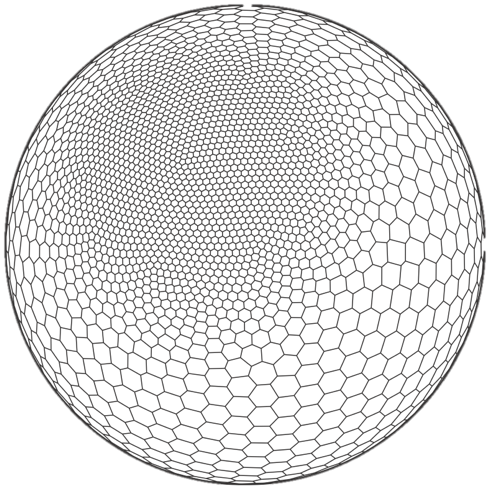
\includegraphics[width=2in]{CentroidalVoronoiTessellation.png}
\end{center}
\caption{A constrained centroidal Voronoi tessellation with localized grid density that could be employed in the MPAS model.} \label{fig:CCVT}
\end{figure}

\subsection{Octahedral reduced Gaussian grid}
\label{subsection:octahedralreducedgaussiangrid}

As with the classical reduced Gaussian grid of \cite{hortalsimmonsMWR1991}, the octahedral 
reduced Gaussian grid \citep{malardel2016,smolarkiewiczetalJCP2016} specifies the latitudes according to the 
roots of the Legendre polynomials. 
The two grids differ in the arrangement of the points along the latitudes, which follows a simple
rule for the octahedral grid: starting with 20 points on the first latitude around the poles, four points 
are added with every latitude towards the equator, whereby the spacing between points along the 
latitudes is uniform and there are no points at the equator. The octahedral reduced Gaussian grid 
is suitable for transformations involving spherical harmonics, and has been introduced for global 
medium-range numerical weather prediction with the spectral dynamical core of the IFS at ECMWF in 2016. 
Figure~\ref{fig:octahedralgrid} depicts the octahedral reduced Gaussian grid nodes together with
the edges of the primary mesh as applied in the context of the finite-volume discretisation of FVM (Section~\ref{sec:FVM}). 


\begin{figure}
\centering
\begin{subfigure}{.4\textwidth}
  \centering
  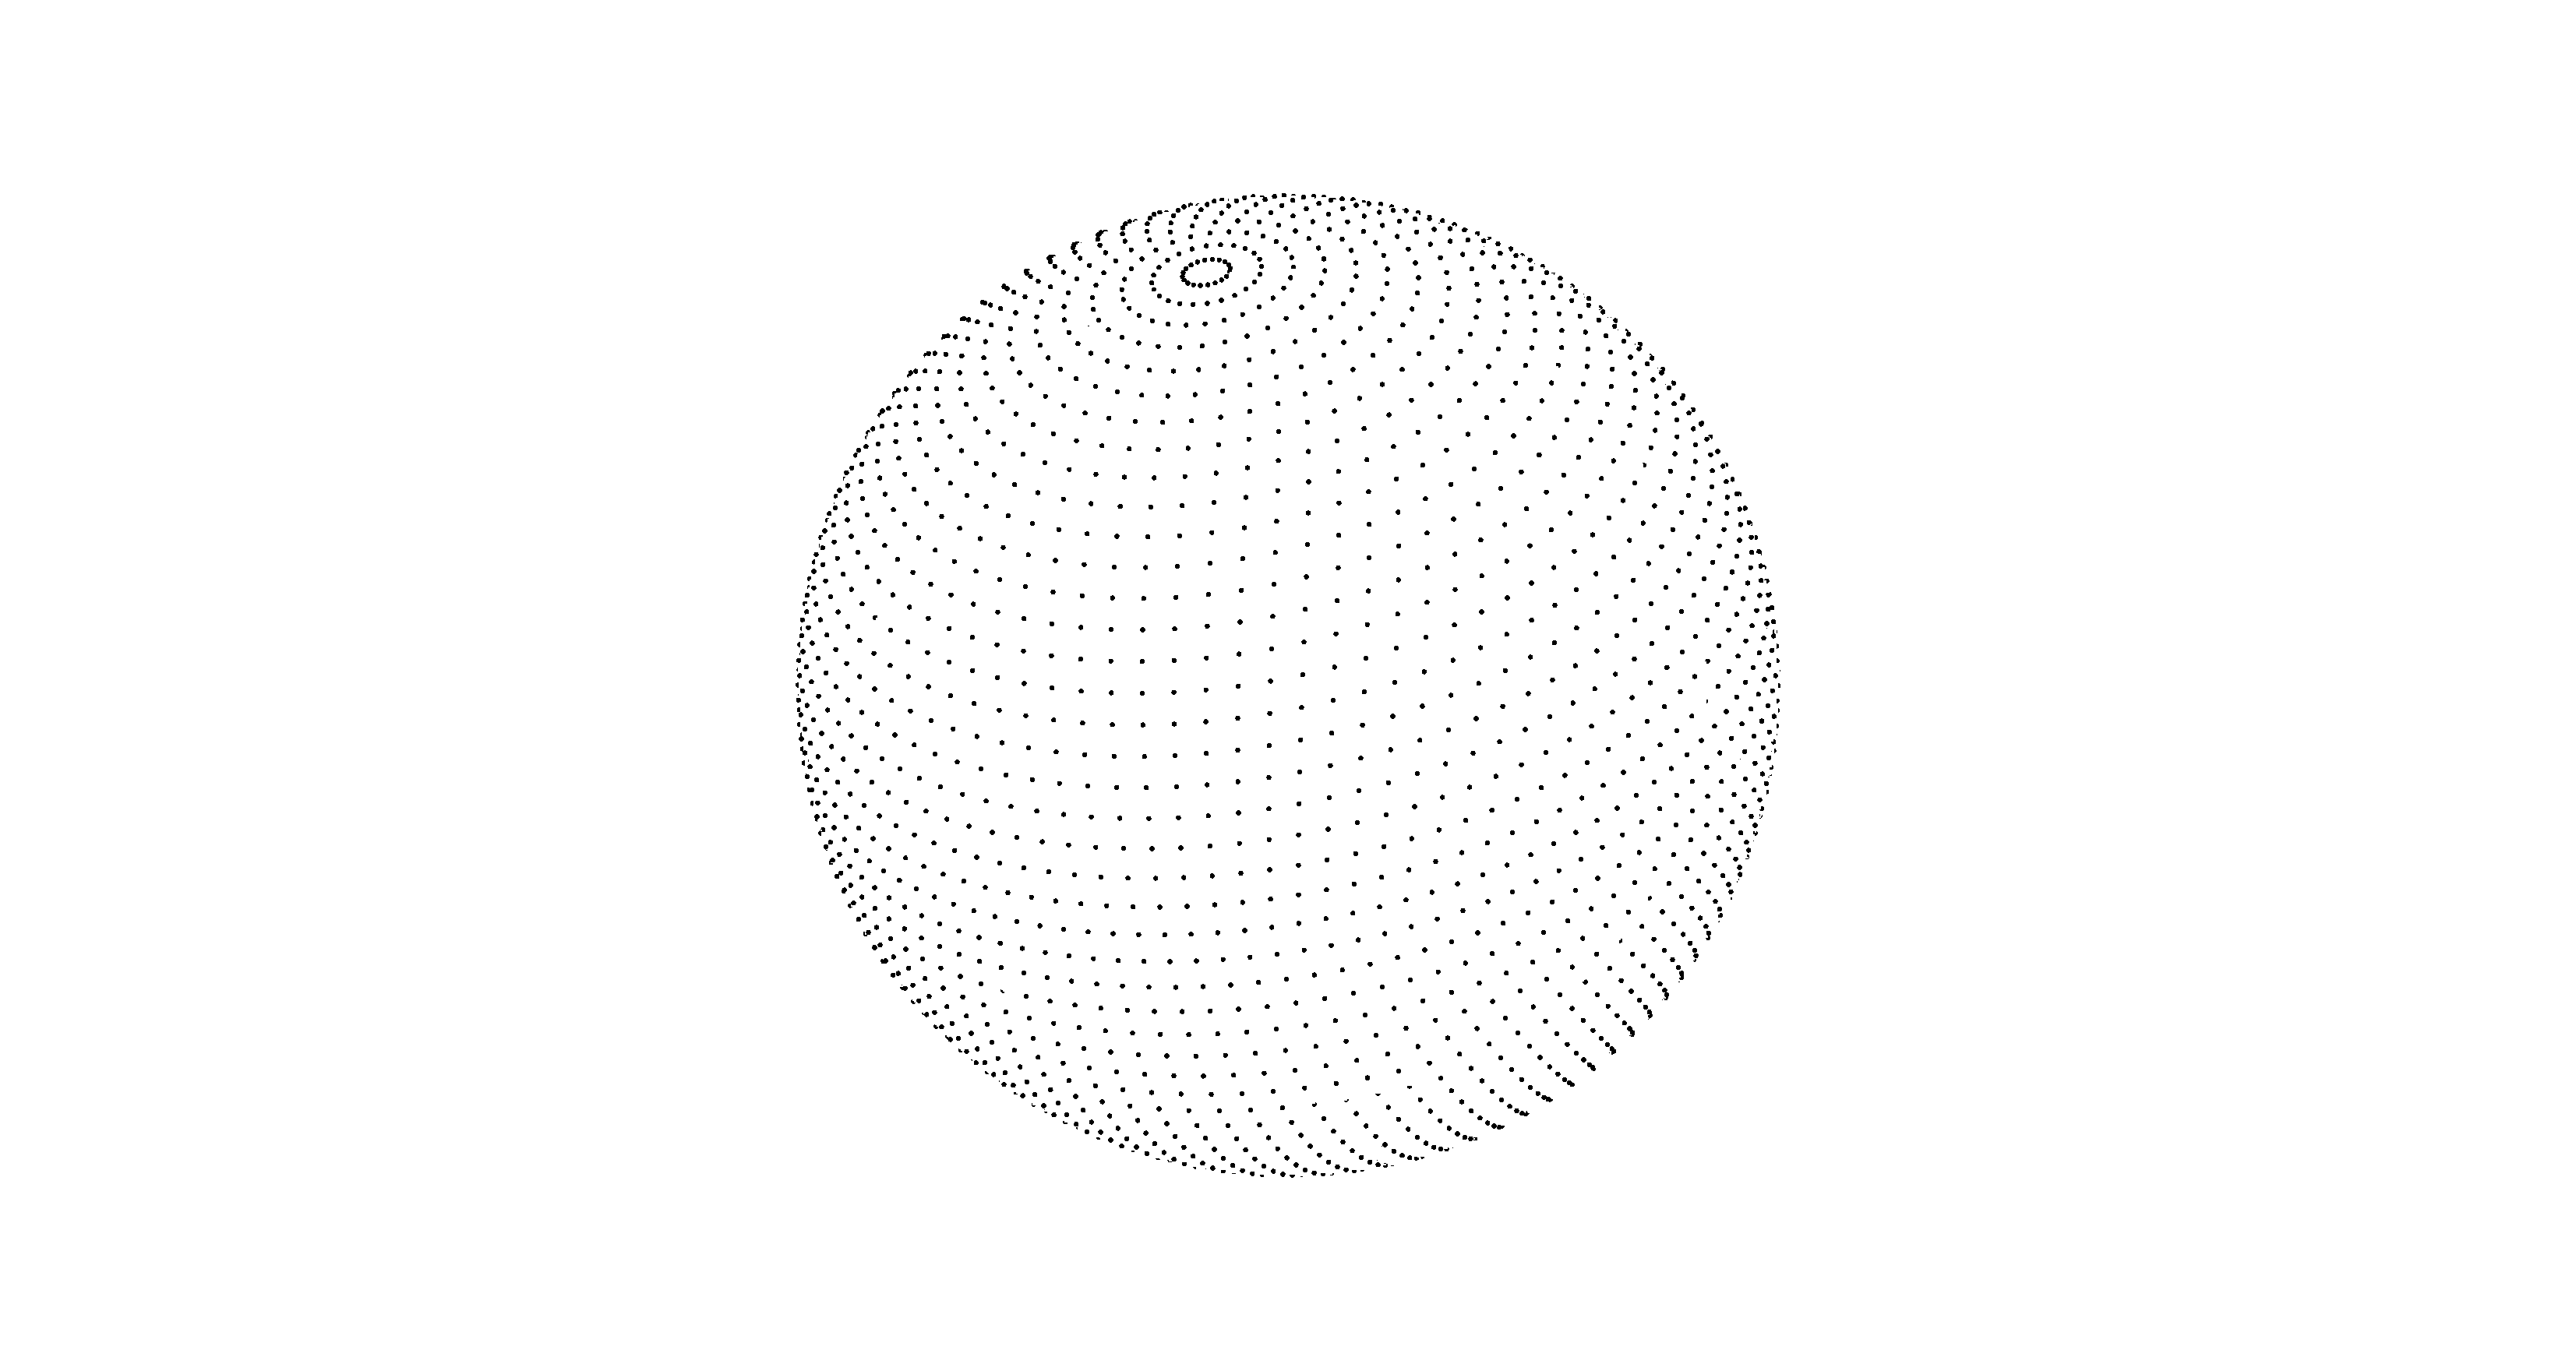
\includegraphics[width=5cm]{contributions/FVM/octahedral_gauss_nodes}
 \end{subfigure}%
\begin{subfigure}{.4\textwidth}
  \centering
  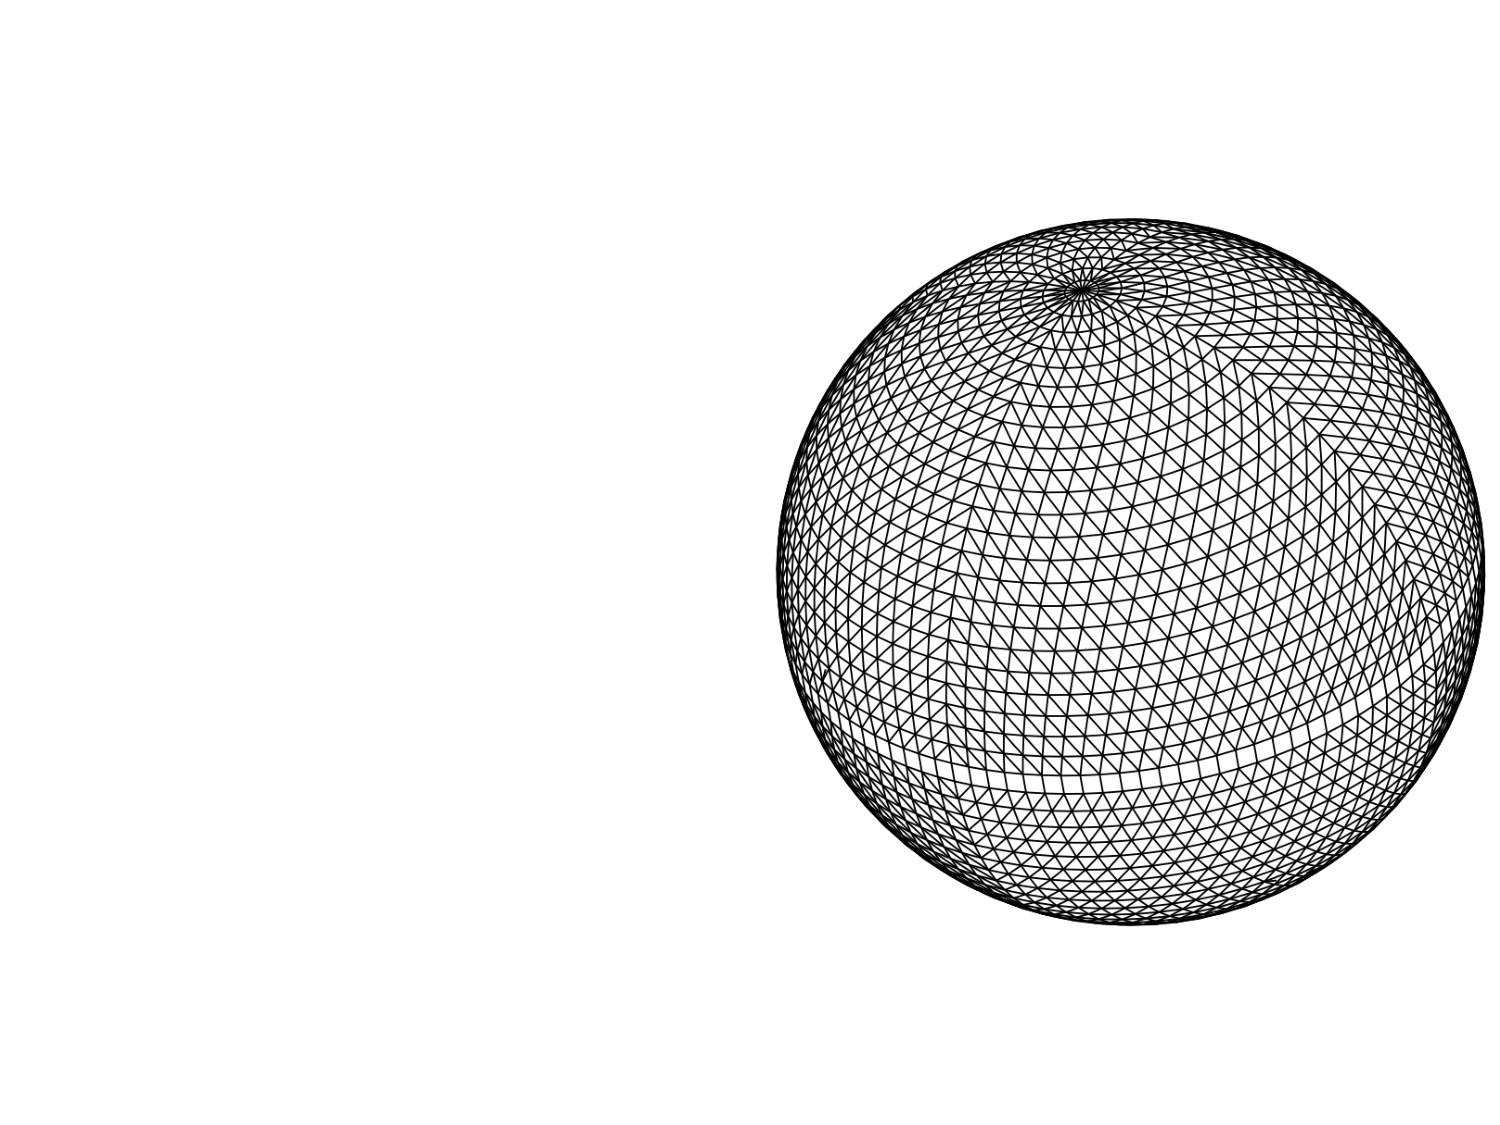
\includegraphics[width=4.7cm]{contributions/FVM/octahedral_RGG_white}
 \end{subfigure}
\caption{Locations of the octahedral reduced Gaussian grid nodes (left), and the edges of the primary mesh 
connecting the nodes as applied with the finite-volume discretisation in FVM (right). A coarse grid with only
24 latitudes between pole and equator is used for illustration. The dual mesh resolution of the octahedral
reduced Gaussian grid is about a factor 2 finer at the poles than the equator; see \cite{smolarkiewiczetalJCP2016}.}
\label{fig:octahedralgrid}
\end{figure}


\subsection{Yin-Yang grid} \label{sec:GEM_model_grid}

The overset Yin-Yang grid \citep{kageama2004yinyang} has two Cartesian grid components (subsets of a latitude-longitude grid) which are geometrically identical (see Figure \ref{fig:gem_yinyang}).  These components are combined to cover a spherical surface with partial overlap along their borders.  The Yin component covers the latitude-longitude region
\begin{equation}\label{eq:gem_yinyang}
(-\frac{\pi}{4}-\delta_{\theta} \leq \theta \leq
\frac{\pi}{4}+\delta_{\theta})  \cap
(-\frac{3\pi}{4}-\delta_{\lambda} \leq \lambda \leq
\frac{3\pi}{4}+\delta_{\lambda}),
\end{equation} where $\delta_{\lambda}, \delta_{\theta}$ are small buffers that are proportional to the respective grid-spacings and are required to enforce a minimum overlap in the overset methodology.  For instance, a common configuration employed by the GEM model for DCMIP fixes 
$ \delta_{\theta}=2 $ degrees and $ \delta_{\lambda}=3 \delta_{\theta}$.  The Yang component covers an analogous area, but is rotated so as to cover the region of the sphere outside of the Yin grid.  This grid is employed by the GEM model, utilizing a pair of regional climate models on the two Cartesian patches.

\begin{figure}[]
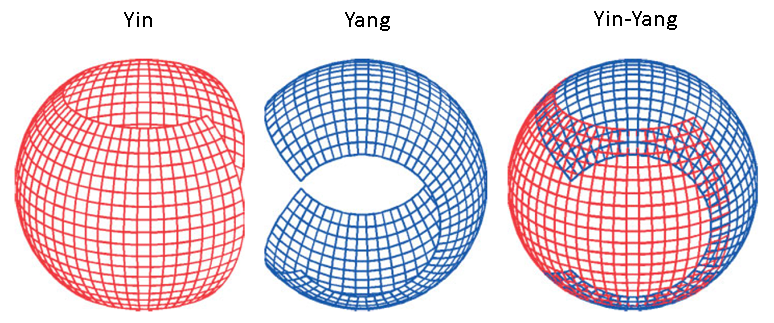
\includegraphics[height=6cm]{gem_yinyang.png}
\caption{ Yin-Yang grid }
\label{fig:gem_yinyang}
\end{figure}

%%%%%%%%%%%%%%%%%%%%%%%%%%%%%%%%%%%%%%%%%%%%%%%%%%%%%%%%%%%%%

\section{Moist Nonhydrostatic Equation Sets} \label{sec:EquationSets}

In this section we describe the fluid equations utilized by nonhydrostatic models.  The material derivative is used for  quantities in the Lagrangian frame (following individual air parcels), and is given by
\begin{align}
\diff{}{t} = \pdiff{}{t} + \vb{u} \cdot \nabla.
\end{align}  Note that tracer variables $q_i$, including specific humidity $q$, satisfy the simple Lagrangian relationship
\begin{align} \label{eq:TracerTransport}
\diff{q_i}{t} = 0.
\end{align}  


\subsection{Diagnostic relationships}

The atmospheric fluid is assumed to be an ideal gas.  For moist air, the ideal gas constant $R^\ast$, specific heat capacity at constant pressure $c_p^\ast$ and specific heat capacity at constant volume $c_v^\ast$ are given by
\begin{align}
R^\ast =& R_d + (R_w - R_d) q, & c_p^\ast =& c_{pd} + (c_{pw} - c_{pd}) q, & c_v^\ast =& c_{vd} + (c_{vw} - c_{vd}) q.
\end{align}  Note that in many models, $R^\ast$, $c_p^\ast$ and $c_v^\ast$ are approximated by $R_d$, $c_{pd}$ and $c_{vd}$, respectively.  Dry air, water vapor and moist air quantities all satisfy the linear relationship $R = c_p - c_v$.  For a two-fluid system (dry air plus water vapor), two independent variables plus the specific humidity $q$ are needed to describe the thermodynamic state of the system.  Key thermodynamic variables include dry air density $\rho_d$, moist density $\rho$, pressure $p$, vapor pressure $e$, temperature $T$, virtual temperature $T_v$, Exner pressure $\pi$, potential temperature $\theta$, and virtual potential temperature $\theta_v$.  Common ratios $\kappa = R^\ast / c_p^\ast$, $\epsilon = R_d / R_w$, and $\gamma = c_p^\ast / c_v^\ast$ are adopted here.

Relationships between key thermodynamic variables arise from the ideal gas law, along with definitions of Exner pressure, potential temperature and virtual potential temperature
\begin{align} \label{eq:DiagnosticRelationships1}
p =& \rho R_d T_v, & \pi =& \left( \frac{p}{p_0} \right)^{\kappa}, & \theta =& T \left( \frac{p_0}{p} \right)^{\kappa}, & \theta_v =& T_v \left( \frac{p_0}{p} \right)^{\kappa},
\end{align}  which further give rise to
\begin{align}
p =& \left( \frac{\rho R_d \theta_v}{p_0^\kappa} \right)^{\kappa - 1}, & \pi =& \left( \frac{\rho R_d \theta_v}{p_0} \right)^{- R^\ast / c_v^\ast}, & \theta =& \frac{T}{\pi}, & \theta_v =& \frac{T_v}{\pi}.
\end{align}

Note that virtual temperature is typically approximated by
\begin{align}
T_v \approx& T \left(1 + \frac{(1-\epsilon)}{\epsilon} q \right),
\end{align} which arises from the exact relationship
\begin{align}
T_v = \frac{T}{1 - \frac{e}{p} (1 - \epsilon)},
\end{align} upon applying $e/p = q / \epsilon$ and using a Taylor expansion around $q = 0$.

\subsection{Prognostic equations for thermodynamic variables}

Note that, as a consequence of (\ref{eq:TracerTransport}), the following simplifications can be applied:
\begin{align}
\frac{1}{T_v} \diff{T_v}{t} =& \frac{1}{T} \diff{T}{t}, & \diff{R^\ast}{t} =& 0, & \diff{c_p^\ast}{t} =& 0, & \diff{c_v^\ast}{t} =& 0.
\end{align}

Mass conservation is typically represented through the continuity equation, which can be written in the Lagrangian frame as
\begin{align} \label{eq:ContinuityEquation}
\diff{\rho}{t} =& - \rho \nabla \cdot \vb{u},
\end{align} or equivalently in the Eulerian frame,
\begin{align}
\pdiff{\rho}{t} =& - \nabla \cdot (\rho \vb{u}).
\end{align}

Further prognostic relationships can be derived from the thermodynamic equation, including the diabatic heating rate $J$,
\begin{align}
\frac{1}{T} \diff{T}{t} - \frac{\kappa}{p} \diff{p}{t} =& \frac{J}{c_p^\ast},
\end{align} which can be alternatively written as
\begin{align}
\diff{\theta}{t} = \frac{J \theta}{c_p^\ast}, \quad \mbox{or} \quad \diff{\theta_v}{t} = \frac{J \theta_v}{c_p^\ast}.
\end{align}  These equations can then be combined with (\ref{eq:ContinuityEquation}) to obtain
\begin{align}
\pdiff{}{t} (\rho \theta_v) + \nabla \cdot (\rho \theta_v \vb{u}) = \frac{J \rho \theta_v}{c_p^\ast},
\end{align} or similarly for $\theta$.  In conjunction with the material derivative of the ideal gas law,  
\begin{align}
\frac{1}{p} \diff{p}{t} = \frac{1}{\rho} \diff{\rho}{t} + \frac{1}{T_v} \diff{T_v}{t},
\end{align} the thermodynamic equation can be written in the form
\begin{align}
\frac{c_v^\ast}{R^\ast T_v} \diff{T_v}{t} - \frac{1}{\rho} \diff{\rho}{t} = \frac{J}{R^\ast}.
\end{align}  Then substituting (\ref{eq:ContinuityEquation}) gives a prognostic equation for virtual temperature,
\begin{align}
\frac{c_v^\ast}{R^\ast} \diff{T_v}{t} + T_v \nabla \cdot \vb{u} = \frac{J T_v}{R^\ast}.
\end{align}  The prognostic equation for temperature is identical except with $T$ substituted for $T_v$.  An analogous equations for pressure can be obtained through a similar procedure,
\begin{align} \label{eq:PressurePrognosticEq}
\frac{c_v^\ast}{c_p^\ast} \diff{p}{t} + p \nabla \cdot \vb{u} = \frac{J p}{c_p^\ast}.
\end{align}  And similarly for Exner pressure,
\begin{align}
\frac{c_v^\ast}{R^\ast} \diff{\pi}{t} + \pi \nabla \cdot \vb{u} = \frac{J \pi}{c_p^\ast}.
\end{align}

\subsection{Momentum Equations}

In coordinate-invariant form the prognostic velocity equations may be written in either the Lagrangian or Eulerian frame as
\begin{align} \label{eq:PrognosticVelocity1}
\diff{\vb{u}}{t} = \pdiff{\vb{u}}{t} + \vb{u} \cdot \nabla \vb{u} = - \frac{1}{\rho} \nabla p - 2 \vg{\Omega} \times \vb{u} - \nabla \Phi,
\end{align} where $\vg{\Omega}$ denotes the planetary vorticity vector and $\Phi$ is the geopotential function.  The three terms on the right-hand-side of this expression correspond to pressure gradient, Coriolis, and gravitational force, respectively.  In Eulerian form one must be careful with the treatment of the momentum advection term $\vb{u} \cdot \nabla \vb{u}$, since for an arbitrary coordinate frame will give rise to Christoffel symbols associated with derivatives of the vector basis {\color{red}[citation needed]}.  Note that it is common to rewrite the pressure gradient force using the relationship
\begin{align}
- \frac{1}{\rho} \nabla p = - c_p^\ast \theta_v \nabla \pi,
\end{align} which follows from (\ref{eq:DiagnosticRelationships1}).  A second form of (\ref{eq:PrognosticVelocity1}) emerges on substituting the vector calculus identity
\begin{align}
\vb{u} \cdot \nabla \vb{u} =& \nabla K + \vg{\zeta} \times \vb{u},
\end{align} where $K = \frac{1}{2} (\vb{u} \cdot \vb{u})$ is the 3D Kinetic energy and $\vg{\zeta} = \nabla \times \vb{u}$ is the 3D relative vorticity vector.  This gives rise to the vector-invariant form,
\begin{align} \label{eq:PrognosticVelocity2}
\pdiff{\vb{u}}{t} = - \frac{1}{\rho} \nabla p - (\vg{\zeta} + 2 \vg{\Omega}) \times \vb{u} - \nabla (K + \Phi). 
\end{align}  Because no gradients of vectors appear in this equation, it avoids derivatives of the coordinate basis that would emerge in (\ref{eq:PrognosticVelocity1}).  In conjunction with (\ref{eq:ContinuityEquation}), both (\ref{eq:PrognosticVelocity1}) also give rise to the flux-form momentum equations,
\begin{align}
\pdiff{}{t} (\rho \vb{u}) = - \nabla \cdot (\vb{u} \otimes \vb{u} + \mathcal{I} p) - 2 \vg{\Omega} \times (\rho \vb{u}) - \rho \nabla \Phi,
\end{align} where $\vb{u} \otimes \vb{u}$ denotes the outer product and $\mathcal{I}$ is the identity matrix.

The equations above still provide some flexibility with regards to the choice of $\Phi$ and $\vg{\Omega}$.  For \textit{deep atmosphere} models, one typically chooses
\begin{align}
\Phi = \frac{g r^3}{3 a^2}, \quad \mbox{and} \quad \vg{\Omega} = \Omega ( \vb{k} \sin \phi + \vb{j} \cos \phi),
\end{align} where $g$ is gravitational acceleration at the surface, $r$ is the radial coordinate, $a$ is the radius of the planet, $\Omega$ is the rotation rate (in s$^{-1}$), $\phi$ is the latitude, $\vb{j}$ is the unit vector oriented in the meridional direction, and $\vb{k}$ is the unit vector oriented in the vertical direction.  For \textit{shallow atmosphere} models, these expressions take the simpler form
\begin{align}
\Phi = g z, \quad \mbox{and} \quad \vg{\Omega} = \Omega \sin \phi \vb{k},
\end{align} where $z$ is the altitude above the surface.  In this case we write $2 \vg{\Omega} = f \vb{k}$, where $f = 2 \Omega \sin \phi$ is the Coriolis parameter.

\subsection{Conservation of Energy}

\subsection{Discretization}



Horizontal momentum equations:

Lagrangian form:
\begin{align}
\diff{\vb{u}_h}{t} + f \vb{k} \times \vb{u}_h + \frac{1}{\rho} \nabla_s p + \nabla_s \phi = 0.
\end{align}

Clark form:
\begin{align}
\pdiff{\vb{u}_h}{t} + \nabla_h (K + \phi) + (\zeta + f) \vb{k} \times \vb{u}_h + \ldots + \dot{s} \nabla_h \left( \pdiff{z}{s} w \right)
\end{align}

Vertical velocity:
\begin{align}
\diff{w}{t} = 
\end{align}

\subsection{Discretization}

The equations in this section make no assumptions about the horizontal coordinate frame, and are written in terms of an arbitrary vertical coordinate $s(t,x,y,z)$.  In this context, the material derivative takes the form
\begin{align}
\diff{}{t} = \pdiff{}{t} + \vb{u}_h \cdot \nabla_s + \dot{s} \pdiff{}{s},
\end{align} where $\vb{u}_h$ is the 2D horizontal velocity vector, $\nabla_s$ is the horizontal gradient operator along surfaces of constant $s$, and $\dot{s}$ denotes the flow velocity perpendicular to surfaces of constant $s$, which relates the physical velocity components $\vb{u}_h$ and $w$ via
\begin{align}
\dot{s} = \diff{s}{t} = \pdiff{s}{t} + \vb{u}_h \cdot \nabla_z s + w \pdiff{s}{z},
\end{align} where $\nabla_z$ is the horizontal gradient operator along surfaces of constant $z$.  

\subsection{FV$^3$} \label{sec:FV3Equations}

%%%GFDL start
FV$^3$ solves the fully-compressible shallow-atmosphere Euler equations using the vector-invariant equations for horizontal momentum on a mass-based Lagrangian vertical coordinate \citep{L2004MWR}. 
%%%GFDL end

\subsection{FVM} \label{sec:FVMEquations}

The fully compressible Euler equations solved in FVM are given as
\begin{subequations} \label{fvm:compressible}
\begin{align}
 & \pdiff{\mathcal{G}\rho_d}{t} + \nabla \cdot \left(\mathbf{v} \mathcal{G} \rho_d\right) = 0~,
\label{fvm:mass}  \\
& \pdiff{\mathcal{G} \rho_d \mathbf{u}}{t} + \nabla \cdot \left(\mathbf{v} \mathcal{G} \rho_d \mathbf{u} \right) = 
\mathcal{G}\rho_d\left( - \Theta \mathbf{\widetilde{G}} \nabla \phi' - \frac{ \mathbf{g}}{\theta_{a}} \left(\theta'+\theta_a (\epsilon q'_v - q_c - q_r) \right)
- \mathbf{f} \times \left( \mathbf{u} - \frac{\theta}{\theta_a} \mathbf{u}_{a} \right) 
+ \mathbf{M} \right)~,
\label{fvm:momentum} \\
%- \frac{L}{c_p \pi} & \Big( \frac{\Delta q_{vs}}{\Delta t} & + E_r  \Big)
& \pdiff{\mathcal{G}\rho_d \theta'}{t} + \nabla \cdot \left(\mathbf{v}\mathcal{G}\rho_d\,\theta' \right) = 
\mathcal{G}\rho_d\left(-\mathbf{\widetilde{G}}^{T}\mathbf{u} \cdot \nabla \theta_{a}
- \frac{L}{c_p \pi} \left( \frac{\Delta q_{vs}}{\Delta t}  + E_r  \right) %\left(C_d + E_p\right) 
+  \mathcal{H} \right)~,
\label{fvm:thermodynamic} \\
& \phi' = c_{p} \theta_{0} \left[\left( \frac{R_{d}}{p_{0}} \rho_d \theta (1+q_v/\varepsilon) \right)^{R_{d}/c_{v}} - \pi_{a} \right]~,
\label{fvm:gaslaw}
\end{align}
\end{subequations}
which describe the conservation laws of dry mass \eqref{fvm:mass}, momentum \eqref{fvm:momentum},
and dry entropy \eqref{fvm:thermodynamic}.
Dependent variables in \eqref{fvm:compressible} are dry density $\rho_d$, three-dimensional 
physical velocity vector $\mathbf{u}$, potential temperature perturbation $\theta'$, and Exner 
pressure perturbation $\pi'$, 
with the thermodynamic variables related by the gas law 
\eqref{fvm:gaslaw}~\footnote{Note that $\phi'$ represents a normalised Exner pressure perturbation.}.
Mixing ratios of water vapor, cloud condensate, and rain are denoted as $q_v$, $q_c$, and $q_r$,
respectively. All primed variables correspond to deviations from an ambient state (denoted by
subscript "a")  that satisfies 
a balanced subset of \eqref{fvm:compressible}, thus $\psi'=\psi-\psi_a$, where $\psi = u,v,w,\theta,..$~;
see \cite{prusa2008} and \cite{smolarkiewiczJCP2014}. 
The subscript "0" appearing with $\theta_0$ refers to a constant reference value. 
Symbols appearing on the rhs of the momentum equation \eqref{fvm:momentum}  are the
coefficient 
\begin{equation}
\Theta := \frac{\theta\,(1+q_v/\varepsilon)}{\theta_0\,(1+q_t)} %\equiv \frac{\theta_d}{\theta_0}~,
\end{equation}
in front of the pressure gradient term with $\Theta/\theta_0$ the density potential temperature,
the gravity vector $\mathbf{g} \equiv (0,0,-g)$~\footnote{In the shallow- versus deep-atmosphere 
form of the governing equations,  gravity is constant $g \equiv g_c$ or varies with height as 
$g = g_c\,(a/r)^2$, respectively.}, the Coriolis parameter $\mathbf{f}$, and  
$\epsilon=1/\varepsilon-1$ with $\varepsilon = R_d/R_v$. % and $\Upsilon_{C} := {\theta}/{\theta_a}$.
The governing equations \eqref{fvm:compressible} are formulated with respect to a geospherical 
coordinate system and a generalised height-based terrain-following vertical coordinate~\footnote{For
simplicity, the vertical coordinate is assumed to be time-independent in the current presentation.}.
Associated symbols are the Jacobian of the metric tensor $\mathcal{G}$, a matrix of metric coefficients
$\widetilde{\mathbf{G}}$, its transpose $\widetilde{\mathbf{G}}^{T}$, 
and the transformation of the physical to the contravariant velocity 
$\mathbf{v} = \mathbf{\widetilde{G}}^{T}\mathbf{u}$; see \cite{prusa2003} and \cite{kuehnleinJCP2012} for discussion.
%(see \eqref{prusa2003,kuehnleinJCP2012} for discussion). 
The symbol $\mathbf{M}$ in \eqref{fvm:momentum} subsumes metric forces due to the curvature
of the sphere \citep[][]{smolarkiewiczetalJCP2016} and momentum dissipation, whereas $\mathcal{H}$ 
in \eqref{fvm:thermodynamic} represents the diffusion of heat. 

%$\mathbf{M}$ and $\mathcal{H}$ subsume various rhs forcings to the
%momentum \eqref{fvm:momentum} and thermodynamic \eqref{fvm:thermodynamic} equations.

\subsection{GEM} \label{sec:GEM_equations}
The equations of GEM model \citep{Girard2014} written out for a log-hydrostatic-pressure like coordinate $\zeta$  system co-rotating with the earth are:
\begin{eqnarray}
\frac{ {d \bf V}_{h} }{dt}+ f {\bf k} \times {\bf{V}_{h}} + R_d T_v\nabla
_\zeta \,  \ln\, p+ \left( 1 + \mu \right) \nabla
_\zeta {\phi} = 0,
\label{eq:gem_eq_1} \\
\frac{d w}{dt}- g \mu = 0,
\label{eq:gem_eq_2} \\
\frac{d}{dt} \ln \left( \pi \pdiff{\ln \pi}{\zeta}\right)
+ \nabla
_{ \zeta }\cdot {\bf V}_{{h}}+\frac{\partial
\dot{ \zeta }}{\partial
\zeta }  = 0,
\label{eq:gem_eq_3} \\
\frac{d \ln T_v}{dt} - \kappa \frac {d \ln p} {dt}=0,
\label{eq:gem_eq_4} \\
R_dT_v+  \frac{p}{\pi} \frac{\partial \phi}{\partial \ln \pi}=0,
\label{eq:gem_eq_5} \\
\frac{d \phi}{dt}-  g w  = 0,
\label{eq:gem_eq_6} \\
1+ \mu - \frac{p}{\pi}   \frac{\partial \ln p}{\partial \ln  \pi}=0,
\label{eq:gem_eq_7} \\
\ln \pi= \zeta+Bs ,
\label{eq:gem_eq_8}
\end{eqnarray}

\noindent with horizontal velocity ${\bf V}_h$, 
generalized vertical velocity $\dot{ \zeta }=\frac{d\zeta}{dt}$, 
vertical velocity $w$,
geopotential $\phi$, 
virtual temperature $T_v$, 
pressure $p$ and
hydrostatic pressure $\pi$. The variable 
$\mu$ is a measure of departure from hydrostatic balance, 
$s$ is related to the surface pressure $\pi_s$ and $B$ is a metric term. The last two variables are defined in (\ref{eq:gem_zeta}).


\subsection{ICON} \label{sec:ICONEquations}

The equation system of the ICON model is based upon the prognostic variables suggested by \cite{gassmann2008} 
but uses the two-dimensional rather than the three-dimensional Lamb transformation to convert the nonlinear momentum
advection into a vector-invariant form. So far, the shallow-atmosphere approximation is applied, but there
are plans to add an option for the unapproximated deep-atmosphere equations. The basic equation system reads as follows
\begin{align}\label{1eqmo}
\pdiff{v_n}{t} + \pdiff{K_h}{n} + (\zeta + f)v_t + w\pdiff{v_n}{z} = -c_{pd} \theta_v \pdiff{ \pi}{n} + F(v_n)
\end{align}
\begin{align}\label{3eqmo}
\pdiff{w}{t} + {\bf v_h} \cdot \nabla w + w \pdiff{w}{z} = -c_{pd} \theta_v \pdiff{\pi}{z} - g  
\end{align}
\begin{align}\label{conteq}
\pdiff{\rho}{t} + \nabla \cdot ({\bf v} \rho) = 0
\end{align}
\begin{align}\label{traceq}
\pdiff{\rho q}{t} + \nabla \cdot ({\bf v} \rho q) = S(\rho q)
\end{align}
\begin{align}\label{thdeq1}
\pdiff{\rho \theta_v}{t} + \nabla \cdot ({\bf v} \rho \theta_v) = \tilde{Q}
\end{align}
{As in \cite{gassmann2013},} Eq. (\ref{thdeq1}) is reformulated using the time derivative of
\begin{align}\label{def-exner}
\pi = \left( \frac{R_d}{p_{00}} \rho \theta_v \right)^\frac{R_d}{c_{vd}}
\end{align}
in order to obtain
\begin{align}\label{thdeq}
\pdiff{\pi}{t} + \frac{R_d}{c_{vd}} \frac{\pi}{\rho \theta_v} \nabla \cdot ({\bf v} \rho \theta_v) = \hat{Q} \,,
\end{align}
{which simplifies the implicit numerical treatment of the terms representing vertical sound wave propagation.}
The prognostic variables of the (untransformed) equation system are the horizontal velocity component normal to the triangle edges $v_n$, the
vertical wind component $w$, density $\rho$, and virtual potential temperature $\theta_v$. When coupled with moisture physics,
$\rho$ represents the full air density including liquid and solid hydrometeors. The reconstructed
tangential velocity component is denoted as $v_t$, and in accordance with the model code, it is assumed here that 
$(v_t,v_n,w)$ form a right-handed system. $\bf v_h$ and $\bf v$ denote the horizontal and three-dimensional wind vector,
respectively. The remaining symbols are the vertical vorticity component $\zeta$, 
the Coriolis parameter $f$, the horizontal part of the kinetic energy $K_h = \frac{1}{2} (v_n^2 + v_t^2)$,
the Exner function $\pi$, the specific heat capacities of dry air at constant pressure $c_{pd}$ and volume $c_{vd}$,
the gas constant of dry air $R_d = c_{pd}-c_{vd}$, the gravitational acceleration $g$, {and the reference pressure
$p_{00}$ = 1000 hPa conventionally used for defining the potential temperature.} $\pdiff{}{n}$ denotes a horizontal derivative
in edge-normal direction, i.e. between the two adjacent mass points. Moreover, $F(v_n)$ denotes source
terms for horizontal momentum (to be specified below), and $\tilde{Q}$ and $\hat{Q}$ denote appropriately 
formulated diabatic heat source terms. In the tracer equation $q$ denotes the mixing ration with respect to the full air density $\rho$, and $S(\rho q)$ represents the source term for a tracer $q$.


\subsection{Tempest} \label{sec:TempestEquations}

The continuity, momentum and thermodynamic equations can be written as:
\begin{align}
\pdiff{\rho}{t} &= - \nabla \cdot (\rho \vb{u}), \\
\pdiff{\vb{u}}{t} &= - \nabla (K + \Phi) - \theta \nabla \Pi + \vg{\eta} \times \vb{u}, \\
\pdiff{\theta_v}{t} &= - \vb{u} \cdot \nabla \theta_v,
\end{align} in terms of Kinetic energy $K = \vb{u} \cdot \vb{u}$, geopotential $\Phi = g_c z$ and absolute vorticity $\vg{\eta} = \vg{\zeta} + \vg{\Omega}$, which consists of relative vorticity $\vg{\zeta} = \nabla \times \vb{u}$ and planetary vorticity $\vg{\Omega}$.  The Exner pressure is related to the prognosed density and potential temperature via
\begin{equation} \label{eq:BaseNonhydrostaticEOS}
\Pi = c_p \left( \frac{p_0}{p} \right)^{R_d/c_p} = c_p \left( \frac{R_d \rho \theta_v}{p_0} \right)^{R_d/c_v}.
\end{equation}

\subsection{Height-based coordinates}

{\color{blue}Define Unstaggered, Lorenz and Charney-Phillips staggering here}

\subsection{Mass-based coordinates} \label{sec:GEM_zeta}
The vertical coordinate of GEM model named $ \zeta$ is of a log-hydrostatic-pressure type and is defined by:
\begin{align}\label{eq:gem_zeta}
 \ln \pi= \zeta+B(\zeta) s \, \, ; \, \, B(\zeta) =\left( \frac {\zeta-\zeta_T} {\zeta_s-\zeta_T}\right)^r \,; \, s= \ln ( \frac {\pi_s} {p_{o}}) \,; \, \, p_{o}=1000 \,\, \mbox{hPa},
\end{align}
with $\zeta_T= \ln \pi_T$, $\zeta_s= \ln {p_{o}}$ and where $r$ is a variable exponent providing added freedom for adjusting the thickness of model layers over high terrain.
Figure \ref{fig:gem_charney-phillips} shows the Charney-Phillips grid in GEM model, giving the position occupied by each variable in the vertical domain.
Horizontal velocity ${\bf V}_h$, geopotential $\phi$ and $q=\ln(p/\pi)$ are on momentum levels.
Temperature $T$, vertical velocity $w$,
generalized vertical velocity $\dot{ \zeta }$ and tracers are on thermodynamic levels. 

%----------------------------------------------------
\begin{figure}[]
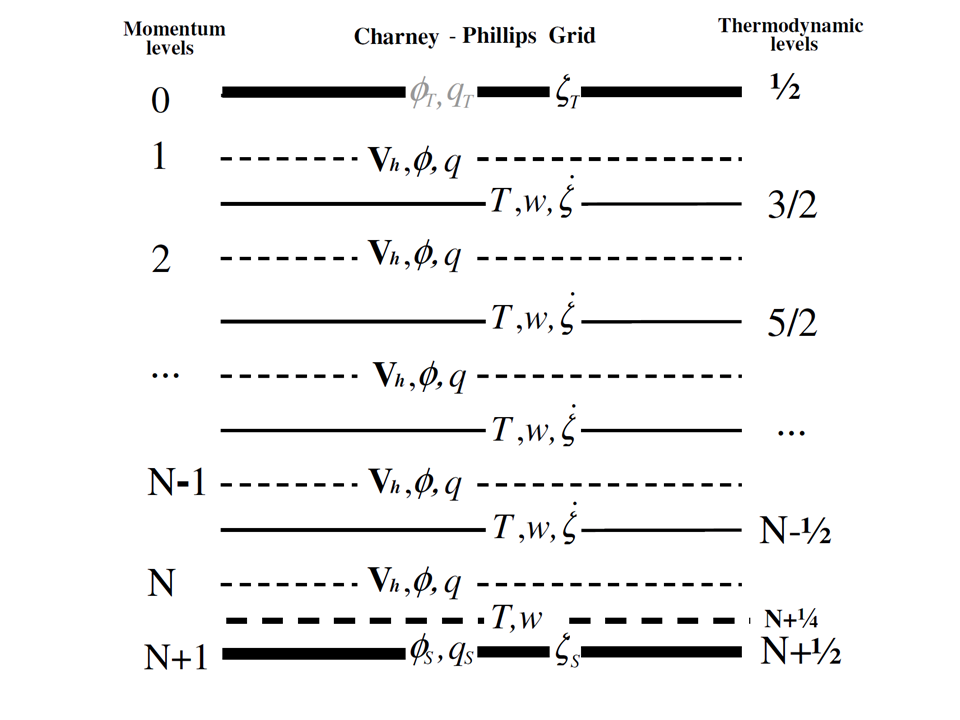
\includegraphics[height=10cm]{gem_charney-phillips.png}
\caption{ Charney-Phillips grid }
\label{fig:gem_charney-phillips}
\end{figure}
%----------------------------------------------------

\subsection{Tracer Transport}

\noindent Lagrangian form:
\begin{align}
\diff{q}{t} &= 0.
\end{align}

\noindent Non-conservative Eulerian form:
\begin{align}
\pdiff{q}{t} &= - \vb{u} \cdot \nabla q.
\end{align}

\noindent Flux form:
\begin{align}
\pdiff{}{t} (\rho q) &= - \nabla \cdot (\rho q \vb{u}).
\end{align}






%%%%%%%%%%%%%%%%%%%%%%%%%%%%%%%%%%%%%%%%%%%%%%%%%%%%%%%%%%%%%

\section{Diffusion and Stabilization} \label{sec:DiffusionStabilization}

{\color{red}[ALL] Include explicit diffusion and stabilization techniques that you have applied in the dynamical core here.}

\subsection{FV3}

Explicit dissipation in FV$^3$ is applied separately to the divergence and to the horizontal fluxes in the governing equations. The D-grid discretization applies no direct implicit dissipation to the divergence, so divergence damping is an intrinsic part of the solver algorithm since otherwise there are no processes by which energy contained in the divergent modes is removed at the grid scale.  FV$^3$ has options for fourth-, sixth-, or eighth-order divergence damping; a second-order option is also available for use in idealized convergence tests, which can be applied in addition to the higher-order diffusion. The monotonicity constraint used in computing the fluxes in the  momentum, thermodynamic, and mass continuity equations is sufficient to damp and stabilize the non-divergent component of the flow. If additional damping is desired, or if the monotonicity constraint has been disabled, there is an option to apply hyperdiffusion to the fluxes in each of these equations, with the exception of the tracer transport, which always uses monotonic transport with no explicit diffusion. This dissipation is of the same order of accuracy as the divergence damping; however the nondimensional coefficient needed is much smaller, usually by at least 3--4 times, than the divergence damping. Both divergence damping and hyperdiffusion are applied along the Lagrangian surfaces and are re-computed every acoustic timestep; there is no explicit damping perpendicular to the Lagrangian surfaces. An option to convert kinetic energy lost to the hyperdiffusion to heat is available. FV$^3$ can also apply a horizontal Smagorinsky eddy diffusion if desired.

A substantial amount of wave absorption is provided by the flexible-lid (constant-pressure) upper boundary;  FV$^3$ also applies second-order diffusion to all fields, except the tracers, to create a sponge layer, typically comprising the top two layers of the domain, to damp other signals reaching the top of the domain. An energy-conserving Rayleigh damping, applied consistently to all three components of the winds, is also available, which is strongest in the top layer of the domain and becomes weaker with distance until reaching a runtime-specified cut-off pressure. 

\subsection{GEM}

Via an application of (\ref{eq:scalar_viscosity_direct}),
scalar viscosity is employed for wind components and tracers. 
A vertical sponge layer, also via an application of (\ref{eq:scalar_viscosity_direct}),
is employed on wind components and $T_v$ with a vertical modulation on the 6 top levels 
and a maximum damping coefficient of $.380000 \times 10^{6}\ \mbox{m\textsuperscript{2}/s}$ at the top.
For stabilization purpose, 
the temporal discretization of GEM presented  
in section \ref{sec:GEM_temporal} uses an off-centering parameter $b^{A} = 0.6$.

\subsection{ICON}

The ICON model employs damping and diffusion operators for numerical stabilization and dynamic closure. Details are described in sections 2.4 and 2.5 of \cite{zangl2014}. Here a brief summary:

\emph{Damping: }In the corrector step a fourth-order divergence damping term $F_{d}(\mathbf{v})$ is applied in order to allow calling the computationally more expensive diffusion operator (see below) at the physics time steps only without incurring numerical stability problems under extreme conditions.
\begin{align}
F_{d}(\mathbf{v}) = - f_d \overline{a_c}^2 \nabla \tilde{\nabla} \cdot \left(\nabla \left(\tilde{\nabla} \cdot v + 
\frac{\Delta }{\Delta z} \left(w-\overline{\overline{w_{cc}}^c}^i \right)\right)\right) \,.
\end{align}
$f_d$ typically attains values between $\frac{1}{1000 \Delta t}$ and $\frac{1}{250 \Delta t}$, and $\overline{a_c}$ is the global mean cell area.

Another artificial damping term is Rayleigh damping on $w$ following \cite{klemp2008}, which serves to prevent unphysical reflections of gravity waves at the model top. The Rayleigh damping is restricted to a fixed number of levels below the model top, and the damping coefficient is given by a hyperbolic tangent.

\emph{Diffusion: }The horizontal diffusion consists of a flow dependent second-order Smagorinsky diffusion of velocity ($F_{D2}(v_n)$) and potential temperature  ($F_{D2}(\theta)$) combined with a fourth-order background diffusion of velocity $F_{D4}(v_n)$.
\begin{align} \label{smagn2}
F_{D2}(v_n) = 4 K_h \tilde{\nabla}^2(v_n)
\end{align}
\begin{align}
F_{D2}(\theta) = a_c \tilde{\nabla} \cdot \left(K_h \frac{\Delta \theta}{\Delta n} \right) \,.
\end{align}
\begin{align}
F_{D4}(v_n) = - k_4 a_e^2 \tilde{\nabla}^2 (\tilde{\nabla}^2(v_n)) \,.
\end{align}
An empirically determined offset of $0.75 k_4 a_e$ is subtracted from $K_h$ in order to avoid excessive diffusion under weakly disturbed conditions.

A fourth-order computational diffusion is also available for vertical wind speed $w$. This filter term is needed at resolutions of O(1 km) or finer because the advection of vertical wind speed has no implicit damping of small-scale structures. Consequently diffusion of $w$ is employed for the DCMIP SCELL test.
\begin{align}
F_{D}(w) = - k_w a_c^2 \nabla^2 (\nabla^2(w)) 
\end{align}

\subsection{Scalar viscosity}

\noindent Scalar viscosity (direct):
\begin{align} \label{eq:scalar_viscosity_direct}
\diff{s}{t} &= \ldots + \nu \nabla \cdot \nabla s.
\end{align}

\noindent Scalar viscosity (conservative):
\begin{align} \label{eq:scalar_viscosity_conservative}
\diff{}{t} (\rho q) &= \ldots + \nu \nabla \cdot ( \rho \nabla q ).
\end{align}

\subsection{Smagorinsky eddy viscosity}

\subsection{Vector viscosity, divergence and vorticity damping}

\noindent Vector viscosity:
\begin{align} \label{eq:vector_viscosity}
\diff{\vb{u}}{t} &= \ldots + \nu \nabla^2 \vb{u}
\end{align}

\noindent Divergence damping:
\begin{align} \label{eq:divergence_damping}
\diff{\vb{u}}{t} &= \ldots + \nu_{div} \nabla (\nabla \cdot \vb{u})
\end{align}

\noindent Vorticity damping:
\begin{align} \label{eq:vorticity_damping}
\diff{\vb{u}}{t} &= \ldots + \nu_{vort} \nabla \times (\nabla \times \vb{u})
\end{align}

\subsection{Hyperviscosity} \label{sec:Diffusion_Hyperviscosity}

{\color{blue}Repeated application of the scalar and vector viscosity operators}

%%%%%%%%%%%%%%%%%%%%%%%%%%%%%%%%%%%%%%%%%%%%%%%%%%%%%%%%%%%%%

\section{Filters and Fixers} \label{sec:FiltersFixers}

{\color{red}[ALL] Include explicit filters and fixers that you have utilized in the dynamical core here.}

\subsection{Mass borrowing (positive definite preservation)}

In GEM model, shape-preserving solutions are computed for tracers by using the quasi-monotone semi-Lagrangian (QMSL) method \citep{Bermejo1992QMSL}. 

\subsection{Mass fixers}

\subsection{Energy fixers}

FV$^3$ has an option to restore lost energy by the adiabatic dynamics, in whole or a fraction thereof (decided by a namelist option at runtime), by globally adding a Exner-function weighted potential temperature increment. This is only done before the physics is called and is not used in idealized simulations. 

%%%%%%%%%%%%%%%%%%%%%%%%%%%%%%%%%%%%%%%%%%%%%%%%%%%%%%%%%%%%%

\section{Temporal Discretizations} \label{sec:TemporalDiscretizations}

{\color{red}[ALL] Describe the time-stepping scheme / temporal discretization employed by your dynamical core here.}

\subsection{Runge-Kutta}

\subsubsection{Ullrich-Kinnmark-Gray 5 step 3rd order scheme} \label{sec:UKG53Scheme}

Explicit terms are evolved using a Runge-Kutta method which supports a large stability bound for spatial discretizations with purely imaginary eigenvalues. This particular scheme is based on \cite{kinnmark1984onestepA, kinnmark1984onestepB} and takes the form
\begin{align}
\psi^{(1)} &= \psi^{(0)} + \tfrac{\Delta t}{5} f(\psi^{(0)}), \nonumber \\
\psi^{(2)} &= \psi^{(0)} + \tfrac{\Delta t}{5} f(\psi^{(1)}), \nonumber \\
\psi^{(3)} &= \psi^{(0)} + \tfrac{\Delta t}{3} f(\psi^{(2)}), \\
\psi^{(4)} &= \psi^{(0)} + \tfrac{2 \Delta t}{3} f(\psi^{(3)}), \nonumber \\
\psi^{(5)} &= -\tfrac{1}{4} \psi^{(0)} + \tfrac{5}{4} \psi^{(1)} + \tfrac{3 \Delta t}{4} f(\psi^{(4)}). \nonumber
\end{align}

\subsection{Semi-implicit time integration of the fully compressible Euler equations in FVM}

In the following we provide an outline of the semi-implicit time stepping scheme for the fully 
compressible Euler equations in FVM (Section~\ref{sec:FVM}). 
A comprehensive discussion of the integration scheme can be found in \cite{smolarkiewiczJCP2014,smolarkiewiczetalJCP2016} 
for dry dynamics; and in \cite{kurowskiJAS2014} and \cite{smolarkiewiczetalMWR2017} for extensions to 
moist dynamics. 
The generic two-time-level second-order template algorithm employed in the integration is given as
\begin{equation}
\psi_{\mbf{i}}^{n+1}= \mathcal{A}_{\mbf{i}}(\widetilde{\psi}^{n},\mathbf{V}^{n+1/2}, (\mathcal{G}\rho_d)^{n}, (\mathcal{G}\rho_d)^{n+1})
+0.5\,\Delta t\,R^{\psi}|_{\mbf{i}}^{\scs n+1}~,
\hspace{1em} \widetilde{\psi}^{n}\,\equiv\,\psi^n+0.5\,\Delta t\,R^{\psi}|^{\scs n}~.
\label{fvm:solscalar}
\end{equation}
In \eqref{fvm:solscalar}, $\psi$ represents the solution variable, $R^{\psi}$ is the respective rhs,
and $\mathcal{A}$ symbolises an advective transport operator assumed here to be the non-oscillatory 
finite-volume MPDATA (Multidimensional Positive Definite Advection Transport Algorithm) scheme 
\citep{smolarkiewiczszmelter2005,kuehnleinJCP2016}~\footnote{Furthermore, 
in \eqref{fvm:solscalar} the vector index $\mathbf{i}$ denotes the spatial position 
on the computational grid, $\Delta t$ is the time step size between levels $n$ and $n+1$.}. 

The integration of the system \eqref{fvm:compressible} can basically be divided into three steps. First, the homogenous
mass continuity equation is integrated with $\psi \equiv \rho_d$, $\mathbf{V} \equiv \mathbf{v}\mathcal{G} $,
and $R^{\rho_d} \equiv 0$ in \eqref{fvm:solscalar}. Second, the thermodynamic \eqref{fvm:thermodynamic}, 
momentum \eqref{fvm:momentum}, and moisture equations enter
\eqref{fvm:solscalar} with $\psi = u, v, w, \theta',...$, $\mathbf{V} \equiv \mathbf{v}\mathcal{G}\rho_d$, and the rhs $R^{\psi}$ 
which is generally depending on all prognostic variables. A high degree of implicitness in the representation of the rhs forcings
is achieved by inverting the overall discrete system \eqref{fvm:solscalar} to obtain closed-form expressions for the
velocity updates -- the procedure is facilitated by the co-located arrangement of variables on the computational mesh. %indicated by the spatial mesh vector index..
Retained on the rhs of the derived closed-form velocity expressions is the pressure gradient term. 
The third step in the solution procedure is to formulate an implicit boundary value problem for the pressure variable $\phi'$ using 
an evolutionary form of the equation of state \eqref{fvm:gaslaw}. An $\mathcal{O}(\Delta t^2)$ integration of this 
equation with a Euler backward template algorithm in the spirit of \eqref{fvm:solscalar} leads a Helmholtz equation. 
The associated 3D elliptic boundary value problem is solved iteratively using a bespoke preconditioned Generalised Conjugate 
Residual approach \citep{smolarkiewiczECMWF2004,smolarkiewiczAG2011}.
Nonlinearities in $R^{\psi}$ and the solution-dependent coefficients of the Helmholtz problem are lagged behind and 
executed in an outer iteration.
 
%The overall integration scheme is 3d implicit with respect to the fast acoustic and buoyant as well as 
%slow rotational modes.


%The integration scheme of FVM approximates the generic conservation law
%\begin{equation}
%\frac{\partial \rho\mathcal{G}\Psi}{\partial t} + \nabla \cdot \left(\rho\mathcal{G}\mathbf{v}  \Psi \right) = \rho\mathcal{G}R^{\Psi}~, %\hspace{1em} 
%\label{scalar}
%\end{equation}
%which represents any of the governing equations \eqref{fvm:mass}-\eqref{fvm:thermodynamic}
%(i.e.~$\Psi = 1 , u, v, w, \theta'$,  as well as corresponding rhs $R^{\Psi}$), by the 
%second-order template algorithm
%\begin{equation}
%\Psi_{\mbf{i}}^{n+1}= \mathcal{A}_{\mbf{i}}(\widetilde{\Psi}^{n},(\rho \mathcal{G} v^{\perp})^{n+1/2}, (\rho\mathcal{G})^{n}, (\rho\mathcal{G})^{n+1})
%+0.5\,\delta t\,R^{\Psi}|

\subsection{Forward-backward vertically-Lagrangian dynamics}

%%%GFDL start

FV$^3$ and its predecessors are integrated using a forward-backwards integration for the Lagrangian dynamics. With the exception of the pressure-gradient force, all of the terms in the momentum, energy, and mass equations are expressable as fluxes, and so can be integrated using the explicit forward-in-time algorithm described by \citet{LR1997QJR}. The horizontal component of the pressure-gradient force is evaluated backwards-in-time using the algorithm of \citet{L1997QJR}; the nonhydrostatic component of the vertical pressure gradient force is evaluated using a semi-implicit solver. This forward-backward timestep is referred to as the ``acoustic'' timestep, although the full solver is advanced on each of these acoustic timesteps. Physics tendencies are applied ``impulsively'' at prescribed intervals, consistent with the forward-in-time discretization; the physics timestep is typically much longer than the acoustic timestep. 
%%%GFDL end

\subsubsection{ICON}

The time stepping scheme of ICON consists of a two-time-level predictor corrector scheme, which is explicit for all terms except for those describing the vertical propagation of sound waves. No time splitting is used with respect to sound waves, because the ration of the maximum wind speed in the mesosphere, which is in part covered by the vertical domain, can be close to one. Instead time splitting is employed to dynamics on the one hand and horizontal diffusion, tracer transport, fast physics on the other hand. Typically a full time step consists of 4 or 5 dynamical sub-steps in which a constant forcing originating from the slow physics is applied. Mass-consistent transport is achieved by passing time-averaged air-mass fluxes from the dynamical sub-steps to the transport scheme.The details of the predictor corrector scheme, including measures to increase the numerical efficiency and to optimize the accuracy, are described in section 2.4 of \cite{zangl2014}. 

\subsection{Semi-Implicit time integration}


%%%%%%%%%%%%%%%%%%%%%%%%%%%%%%%%%%%%%%%%%%%%%%%%%%%%%%%%%%%%%
\subsection { The 2 time level semi-Lagrangian implicit time discretization in GEM model} \label{sec:GEM_temporal}

Consider a frictionless adiabatic prognostic equation of the form:
\begin{equation} 
\frac {dF}{dt}+G=0,
\label{eq:gem_temporal_O}
\end{equation}
\noindent where $F$ represents one of the prognostic variables and $G$ represents the remaining terms, some of which are non-linear.
Based on the semi-Lagrangian scheme,
The equation (\ref {eq:gem_temporal_O}) is discretized as:
\begin{equation} 
\frac{F^A-F^{D}} {\Delta t}+ b^A G^A + (1-b^A) G^D = 0,
\label{eq:gem_temporal_D}
\end{equation}
with $A \, \mbox{(Arrival)} = (\vg{r},t)$, $D \, \mbox{(Departure)} = (\vg{r}-\Delta \vg{r},t-\Delta t)$ 
and $\vg{r}$ is the 3D grid position. 
The displacements $\Delta \vg{r}$ are obtained by the iterative process:
\begin{equation} 
\Delta  \vg{r}^{i} =  \left [ b^A \vg{V}(\vg{r},t) + (1-b^A) \vg{V}(\vg{r}-\Delta \vg{r}^{i-1},t-\Delta t) \right ] \Delta t,
\label{eq:gem_temporal_traj} 
\end{equation} 
where  $\vg{V}$ is the 3D wind vector.
From (\ref {eq:gem_temporal_D}), we regroup unknown terms on the left-hand side 
and known terms on the right-hand side, that is:
\begin{align} 
\frac{F^A} {\tau} + G^A =  \frac{F^{D}} {\tau}- \beta G ^{D}= R,
\label{eq:gem_temporal_AD}
\end{align}
\noindent where $\tau= \Delta t b^A$ and $\beta = (1-b^A)/b^A$. 
Cubic Lagrange interpolation is used for upstream evaluations $(F^{D}, G^{D})$.
Each left-hand side term $\frac{F^A} {\tau}+ G^A$ is then split into a linear part $L$ and a nonlinear residual part $N$:   
\begin{align} 
\frac{F^A} {\tau} + G^A = L + N = R. 
\label{eq:gem_temporal_LN}
\end{align}
The linearization is done around a constant in time, horizontally homogeneous, reference state. 
This results in the non-linear problem:
\begin{align}
L^{i}=R-N^{i-1},
\label{eq:gem_temporal_solve}
\end{align}
which is solved with two iterations.   
In each iteration, the
linear system (\ref{eq:gem_temporal_solve})  
is reduced to an Helmholtz problem 
for one composite variable.
It 
is solved 
with a direct solver
using the Schwarz-type domain decomposition method on Yin-Yang grid \citep{Qaddouri2008schwarz}.
The composite variable solution is used to update the prognostic variables at time $t$.  
Our procedure involves another iterative process linked to the estimation of $\vg{V}(\vg{r},t)$ in the displacement calculations (\ref{eq:gem_temporal_traj}). 
This results in redoing the sequence of operations (\ref{eq:gem_temporal_traj})-(\ref{eq:gem_temporal_solve}). 
At each time step, the cubic Lagrange interpolation is used to update the static halo region of both panels of the Yin-Yang grid 
\citep{Qaddouri2011operational}. 

%%%%%%%%%%%%%%%%%%%%%%%%%%%%%%%%%%%%%%%%%%%%%%%%%%%%%%%%%%%%%

\section{Dynamical Cores}

{\color{red}In this section provide a short description (approximately 0.5 pages) of the dynamical core, focusing on unique features or design specifications.  Do not include information on the physical parameterizations used by the modeling system.  Make reference to the model grid employed from section \ref{sec:ModelGrids}, the specific equation set being discretized by the model in section \ref{sec:EquationSets}, explicit numerical techniques for diffusion and stabilization in section \ref{sec:DiffusionStabilization}, filters and fixers in section \ref{sec:FiltersFixers} and the temporal discretization in section \ref{sec:TemporalDiscretizations}.}

\subsection{Colorado State University Model (CSU)}

The CSU model uses an optimized geodesic grid to discretize the sphere, with height as the vertical coordinate. The model is based on the non-hydrostatic Unified System of equations proposed by Arakawa and Konor (2009), which filters vertically propagating sound waves but allows the Lamb wave and does not require a reference state. The horizontal wind field is determined by predicting the vertical component of the vorticity and the divergence of the horizontal wind, and then solving a pair of two-dimensional Poisson equations for a stream function and velocity potential. Time-differencing is based on the third-order Adams-Bashforth  scheme. Horizontal diffusion is included in the form of a $\nabla^4_z()$ operator acting on the vorticity, divergence, potential temperature, and tracer.  
\subsection{Geophysical Fluid Dynamics Laboratory FV Cubed (GFDL-FV$^3$)}

FV$^3$ uses a fully finite-volume discretization of the fully-compressible nonhydrostatic Euler equations on the equiangular gnomonic cubed-sphere grid on a terrain-following Lagrangian vertical coordinate. The flow is entirely along the Lagrangian surfaces, allowing vertical transport to be represented implicitly without additional advection terms. Fluxes are computed using the Piecewise-Parabolic Method of \citet{CW1984JCP} with an optional monotonicity constraint; in nonhydrostatic applications the monotonicity constraint is used primarily for tracer transport. The discretization is on the C-D grid described by \citet{LR1997QJR} which acts as a simplified Riemann solver: the D-grid winds are interpolated to the C-grid and then advanced by half of an acoustic timestep, giving time-centered winds that can then be used to compute the fluxes and advance the flux terms by a full acoustic timestep. Since divergence is effectively invisible to the solver, a divergence damping is applied to control numerical noise as divergent modes cascade to the grid scale. 

Implicit viscosity is applied through the monotonicity constraint; if non-monotonic advection is used for the momentum and total air mass a weak explicit hyperviscosity is applied for stability and to alleviate numerical noise. Explicit viscosity is applied every acoustic timestep. 

The solver prognoses horizontal winds, in the native Gnomonic local coordinate; virtual potential temperature, which is conserved by the adiabatic dynamics; mass, represented by the difference in hydrostatic pressure between the top and bottom of a grid cell; and tracer mass. The nonhydrostatic solver adds a prognostic vertical velocity and geometric height of each grid cell, which can then be used to compute density. All variables are 3D cell-mean values, except for the horizontal winds, which are 2D face-mean values on their respective staggerings; as a result, vorticity is a 3D cell-mean value.


\subsection{Global Environmental Multiscale (GEM) Model} \label{sec:GEM_core}

In GEM model, we use the Yin-Yang grid and horizontal discretization is done on an Arakawa C grid.
The vertical coordinate $\zeta$ is of a log-hydrostatic-pressure type and vertical discretization is based  
on the Charney-Phillips grid.
A 2 time level semi-Lagrangian implicit time discretization is implemented as described in section \ref{sec:GEM_temporal}. 
A scalar viscosity is employed for wind components and tracers 
via an application of (\ref{eq:scalar_viscosity_direct}). 
Viscosity operations are applied after the completion of the dynamic time step.

\subsection{High-Order Method Modeling Environment (HOMME)}

{\color{red}[HALL]}

HOMME stands for the High Order Method Modeling Environment which provides the framework for the CAM-SE and ACME-Atmosphere dynamical cores along with several experimental versions  including a non-hydrostatic model. It was designed to be mass and energy conserving with nearly optimal parallel scalability at large core counts. The CAM-SE dynamical core is a hydrostatic model that partitions the globe horizontally using an unstructured grid of quadrilateral elements. These elements are arrange by default in a cube-sphere structure, but variable-resolutions grids with conforming edges may also be employed. Each quadrilateral extends in the radial direction to form a column using the shallow-atmosphere approximation $r\approx a$ where $a$ is the mean radius of the Earth. It employs a hybrid terrain-following / pressure coordinate $\eta \in (0,1]$ which transforms smoothly from a pure pressure coordinate at the top of the model to a terrain-following surface-pressure coordinate at the bottom. A conventional vector-invariant form for the moist primitive equations is employed with prognostic zonal and meridional wind components $u,v$, temperature $T$, surface pressure $p_s$, and tracer mixing ratios $q_i$. The PDEs are discretized using a split approximation, with a nodal 4th order spectral element discretization in the horizontal and the mimetic (mass and energy conserving) 2nd order finite difference discretization of \cite{simmons1981energy} in the vertical. Fields are co-located in the horizontal in the sense that they share the same 4th order basis functions. Lorenz staggering is employed in the vertical with (u,v,T,p) placed on layer midpoints while vertical fluxes $m \dot \eta$ are placed on layer interfaces.

A floating Lagrange formulation is used for tracer advection and optionally for the vertical dynamics as well, in which vertical levels are advected with the fluid. After several time-steps, the levels are remapped onto the fixed Eulerian $\eta$ grid in order prevent pressure surfaces from crossing. Several limiter options are available including a sign-preserving limiter and a monotone optimization base limiter described in \cite{guba2014optimization}. Diffusion is applied in the horizontal with a 4th order hyperviscosity operator, decomposed into two applications of the Laplacian operator in divergence / vorticity form. The physics, tracer, dynamics, and vertical remapping schemes are applied in a time split manner with adjustable sub-cycling ratios. Tracer advection is discretize in time with a 3-stage 2nd order strong stability preserving (SSP) scheme of Spitteri and Ruuth \cite{spiteri2002new}. The dynamics are also discretized using one of several explicit Runge-Kutta times schemes. Physics-dynamics coupling may be achieved using a single adjustment at the end of the physics timestep, through tendency update every dynamics step, or by a hybrid of the two.

In addition to the primitive equation model, HOMME also hosts an experimental nonhydrostatic dynamical core which retains many of the features of the traditional CAM-SE model. This model makes use of the shallow-atmosphere Euler equations of motion in terrain-following $\eta$ coordinates, as first described by \cite{laprise1992euler}. In its current incarnation, unstructured spectral elements are retained in the horizontal with matching spectral elements in the vertical. Prognostic variables include the 3d wind velocity components $u,v,w$, the surface pressure $p_s$, potential temperature $\theta$, and geopotential height $\phi$. Fields are current co-located in the vertical and explicit time-stepping is used. Planned improvements call for vertically implicit time stepping, and possible Charney-Phillips staggering. This model has been successfully applied to the dry DCMIP-2012 dynamical core tests including (vertical SE) tracer transport, orogoraphic waves, gravity waves, and the dry baroclinic instability. Moist dynamics, physics/dynamics coupling, and implicit time integration routines are currently under development.

\subsection{ICON}

The ICON model discretizes the compressible equations for a shallow atmosphere in vector invariant form for the horizontal wind on a triangular Arakawa C-grid and a smoothed terrain following height based Lorenz grid. The prognostic variables are the normal wind $v_n$ at the edge mid points of full levels, the vertical wind $w$ in the circumcenters of the triangles on half levels and virtual potential temperature $\theta_v$, full air density $\rho$, which includes moisture and hydrometeor densities and tracer mixing ratios $q_x$ with respect to the full air density. The discretization in time employs a two time level predictor corrector scheme, which is explicit in all terms except for those describing the vertical propagation of sound waves. Time splitting is applied between the dynamics that is forced by slow physics on the one hand and horizontal diffusion, tracer transport, and fast physics. One complete time step typically includes 5 dynamical sub-steps. The average air mass flux of the dynamical  sub-steps is provided to the tracer transport to allow for a mass-consistent transport. For stabilization of the divergence term on the triangular C-grid the divergence in a triangle is computed from modified normal wind components resulting from a weighted average including normal winds on edges of adjacent cells. Further divergence damping is applied to the normal wind at every sub-step. Rayleigh damping is applied to the vertical wind in layers close to the model top in order to avoid the reflection of gravity waves. The horizontal diffusion, which is applied at full model time steps, combines a flow dependent Smagorinski scheme with a background 4th order Laplacian diffusion operator. For tracer transport a flux form semi-Lagrangian scheme with monotone flux limiters is used, which grants local mass conservation and consistency with the air motion. The numerical methods have been chosen for high numerical efficiency, and they rely on next neighbour communication only, thus allowing massive parallelization.

\subsection{Model for Prediction Across Scales (MPAS)}

{\color{red}[SKAMAROCK]}

\subsection{Naval Research Laboratory NEPTUNE Model}

{\color{red}[VINER, REINECKE]}

\subsection{Ocean-Land-Atmosphere Model (OLAM)}

{\color{red}[WALKO]}

\subsection{DYNAMICO}

{\color{red}[DUBOS]}

\subsection{Tempest}

The Tempest model \citep{ullrich2014global, guerra2016high} uses a horizontal spectral element discretization and vertical staggered nodal finite element method based on the cubed-sphere grid with terrain-following height-based coordinate.  The standard Eulerian equations are employed with moist density $\rho$, thermodynamic closure $\theta_v$ and tracer density $\rho q$.  These continuous equations are given in section \ref{sec:TempestEquations}.  The implementation includes both fully explicit time integration, using the UKG53 scheme described in section \ref{sec:UKG53Scheme}, and implicit-explicit options, where horizontal terms are explicitly discretized and vertical terms are treated implicitly.  Scalar hyperviscosity is employed for $\rho$, $\theta$ and tracer variables via repeated application of (\ref{eq:scalar_viscosity_direct}).  Vector hyperviscosity is also applied by decomposing the horizontal vector Laplacian into divergence damping (\ref{eq:divergence_damping}) and vorticity damping (\ref{eq:vorticity_damping}) terms.  Both viscosity operations are applied after the completion of all Runge-Kutta sub-cycles.

\subsection{Finite-volume module of the Integrated Forecasting System}
\label{sec:FVM}

%{\color{red}[KUEHNLEIN]}

The finite-volume module (FVM) of the Integrated Forecasting System (IFS) is developed at 
ECMWF \citep{smolarkiewiczetalJCP2016}. FVM solves the fully compressible Euler 
equations in geospherical coordinates. Both deep-atmosphere and shallow-atmosphere equations 
are available by means of simple switches. The formulation incorporates 
a generalised, optionally time-dependent, terrain-following vertical coordinate based on height. 
A centred two-time-level semi-implicit integration scheme is employed with 3D implicit treatment 
of acoustic, buoyant, and rotational modes \citep{smolarkiewiczJCP2014}. The associated 3D 
Helmholtz problem is solved iteratively using a bespoke preconditioned Generalised 
Conjugate Residual approach. 
The integration procedure uses the multidimensional flux-form Eulerian non-oscillatory MPDATA 
advection scheme \citep{smolarkiewiczszmelter2005,kuehnleinJCP2016}. 
The horizontal spatial discretisation is fully unstructured finite-volume using the 
median-dual approach. This is combined with a structured-grid finite-difference approach in the 
vertical direction; see \cite{smolarkiewiczetalJCP2016} for an exposition. 
In both the horizontal and the vertical discretisation, all prognostic variables are 
co-located. The median-dual finite-volume mesh in the horizontal is developed about the points/nodes 
of the octahedral reduced Gaussian grid (Section~\ref{subsection:octahedralreducedgaussiangrid}). The octahedral 
reduced Gaussian grid is also employed in the spectral dynamical core of the current operational 
IFS at ECMWF, which facilitates interoperability of the two formulations. However, we note that FVM is 
not restricted to this grid and offers capabilities towards a broad classes of meshes including adaptivity. 

No explicit diffusion is applied in FVM for DCMIP, apart from the momentum dissipation and scalar 
diffusion required for some of the test cases, which is the vertical dissipation/diffusion in the planetary
boundary layer parametrisation and the constant-coefficient second-order dissipation/diffusion in 
the supercell test. An absorbing layer in the first latitude ring around the poles is optionally used in 
the form of a Rayleigh-type forcing to the prognostic variables. The dynamics time step is adapted 
at every time step according to a given maximum advective CFL number (typically somewhat smaller 
than 1). The physics time step is identical to the dynamics time step. 
%The first row of the table below refers to the size of the octahedral reduced Gaussian grid, where 
%the number following "O" (for octahedral) denotes the number of latitudes between pole and equator.


%Neither explicit diffusion/filters nor decentering of the time-stepping scheme is applied in DCMIP, 
%No explicit diffusion is applied in FVM in DCMIP, apart from the explicit momentum dissipation and 
%scalar diffusion required for some of the test cases.  FVM uses adaptive time stepping for optimal
%efficiency and accuracy. 
 
%FVM employs distributed- and shared-memory parallelisation using the MPI and OpenMP standards, 
%respectively. %The underlying distributed-memory data structures in FVM are provided by the Atlas 
%framework developed at ECMWF. 

\subsection{Nonhydrostatic ICosahedral Atmospheric Model (NICAM) Model}

{\color{red}[MIURA]}

%%%%%%%%%%%%%%%%%%%%%%%%%%%%%%%%%%%%%%%%%%%%%%%%%%%%%%%%%%%%%

\section{Idealized Physical Parameterizations}

\subsection{Kessler Physics} \label{sec:KesslerPhysics}

The cloud microphysics update according to the following equation set:
\begin{alignat}{5}
\frac{\Delta \theta}{\Delta t} = & - \frac{L}{c_p \pi} & \Big( \frac{\Delta q_{vs}}{\Delta t} & + E_r  \Big) & \\
\frac{\Delta q_v}{\Delta t} = & & \frac{\Delta q_{vs}}{\Delta t} & + E_r \\
\frac{\Delta q_c}{\Delta t} = & & - \frac{\Delta q_{vs}}{\Delta t} & & - A_r & - C_r \\
\frac{\Delta q_r}{\Delta t} = & & & - E_r & + A_r & + C_r & - V_r \pdiff{q_r}{z},
\end{alignat} where $L$ is the latent heat of condensation, $A_r$ is the autoconversion rate of cloud water to rain water, $C_r$ is the collection rate of rain water, $E_r$ is the rain water evaporation rate, and $V_r$ is the rain water terminal velocity.

The pressure follows from the equation of state
\begin{equation}
p=\rho R_dT(1+0.61q_v)
\end{equation} with $p$ the pressure, $\rho$ the density of moist air, $R_d$ the gas constant for dry air, $T$ the temperature and $q_v$ the mixing ratio of water vapor. The equation is rewritten as a nondimensional pressure $\Pi$ equation.
\begin{equation}
\pi = \left(\frac{p}{p_0}\right)^{\frac{R_dT}{cp}}
\end{equation}

To determine the saturation vapor mixing ratio the Teten's formula is used,
\begin{equation}
q_{vs}(p,T) = \left( \frac{380.0}{p} \right) \exp\left(17.27 \times \frac{T-273.0}{T-36.0}\right)
\end {equation}

The autoconvection rate ($A_r$) and collection rate ($C_r$) follow Kessler parametrization and are defined by:
\begin{align}
A_r &= k_1(q_c-a) \\
C_r &= k_2q_cq_r^{0.875}
\end{align} With $k_1=0.001 \text{s}^{-1}$, $a=0.001 \text{g}.\text{g}^{-1}$ and $k_2=2.2 \text{s}^{-1}$ 

Deriving from \cite{klemp1978simulation} description of cloud water,rain water and water vapor mixing ratios. they are define as followed:
\begin{equation}
q_c^{n+1}=\mbox{max}(q_c^r-\Delta q_r,0)
\end{equation}
\begin{equation}
q_r^{n+1}=\mbox{max}(q_r^r-\Delta q_r+S,0)
\end{equation} where $S$ is the sedimentation term and $\Delta q_r$ is defined as
\begin{equation}
\Delta q_r=q_c^n-\frac{q_c^n-\Delta \text{t}\ \mbox{max}(A_r,0)}{1+\Delta \text{t} C_r}
\end{equation}

The Rain evaporation equation is defined similarly to \cite{ogura1971numerical} description:
\begin{equation}
E_r=\frac{1}{\rho}\frac{\left(1-\frac{q_v}{q_{vs}}\right)C(\rho q_r)^{0.525}}{5.4\times10^5+\frac{2.55\times10^6}{pq_{vs}}}
\end{equation}  With ventilation factor C define as 
\begin{equation}
C_r=1.6+124.9(\rho q_r)^{0.2046}
\label{venti}
\end{equation}

The liquid water terminal velocity is similar to \cite{soong1973comparison} description with a mean density adjustment as suggested by \cite{kessler1969distribution}:
\begin{equation}
V_r = 36349(\rho q_r)^{0.1346}\left(\frac{\rho}{\rho_0}\right)^{-\frac{1}{2}}
\end{equation}

%%%%%%%%%%%%%%%%%%%%%%%%%%%%%%%%%%%%%%%%%%%%%%%%%%%%%%%%%%%%%

\section{Surface Fluxes on an Aqua-Planet with Prescribed Sea Surface Temperatures} \label{sec:OceanSurfaceFluxes}

The forcing by surface fluxes from an idealized ocean is described in \cite{reed2012idealized} and is partly reproduced here. We use a model configuration which corresponds to an aqua-planet setup with prescribed sea surface temperatures (SSTs). This forcing by the surface fluxes is applied to the state variables in the lowermost model level using a partially implicit formulation to avoid numerical instabilities.  Throughout this section we use the subscript $a$ to denote variables defined on the lowermost model level.

The surface fluxes depend on the \textit{drag coefficient} $C_d$, defined as
\begin{equation} \label{eq:DragCoefficient}
\begin{array}{ll}
C_d = C_{d0} + C_{d1} \vert \vec{v}_a \vert & \mbox{for $\vert \vec{v}_a \vert < 20$ m s$^{-1}$} \\ 
C_d = 0.002 & \mbox{for $\vert \vec{v}_a \vert \geq 20$ m s$^{-1}$}, 
\end{array}
\end{equation}
where $C_{d0}$ and $C_{d1}$ are $7.0 \times 10^{-4}$ (unitless) and $6.5 \times 10^{-5}$ s m$^{-1}$, respectively, and $\vert \vec{v}_a \vert$ is the magnitude of the horizontal wind at the lowermost model level.  In terms of the zonal wind $u_a$ and meridional wind $v_a$, it is defined as
\begin{equation}
\vert \vec{v}_a \vert = \sqrt{u_a^2 + v_a^2}.
\end{equation}  For both evaporation and sensible heat the bulk coefficient is set to
\begin{equation} \label{eq:BulkTransferCoefficient}
C_E = C_H = 0.0011.
\end{equation}

The formulation of the surface fluxes makes use of the height of the lowermost full model level $z_a$ (in m).  For pressure-based models, $z_a$ can be expressed with the help of the hydrostatic equation in terms of pressure
\begin{eqnarray} \label{eqn:za}
z_a = \frac{R_d T_{\nu,a}}{g} \frac{(\ln p_s- \ln p_-)}{2},
\end{eqnarray}
where $T_{\nu,a} = T_a (1+0.608 q_a)$ is the virtual temperature at the lowermost full model level and $p_-$ is the edge pressure at the model level interface between the lowest and second lowest full model levels. This notation and all following equations assume that the temperature, horizontal wind components and the specific humidity in the physical parameterization package are co-located in both the vertical and horizontal directions, as is the case for the Lorenz grid. The height of the lowest full model level should ideally lie between 60-70m above the ground to make the results comparable to those in the literature.

As described in \cite{reed2012idealized}, the surface fluxes can be written as
\begin{eqnarray}
\frac{\partial \vec{v}_a}{\partial t} &=& - \frac{C_d \vert \vec{v}_a \vert \vec{v}_a}{z_a} \label{sfu} \\
\frac{\partial T_a}{\partial t} &=& \frac{C_H \vert \vec{v}_a \vert (T_s-T_a)}{z_a} \label{sft} \\
\frac{\partial q_a}{\partial t} &=& \frac{C_E \vert \vec{v}_a \vert(q_{sat,s}-q_a)}{z_a}. \label{sfq}
\end{eqnarray}
We note that the wind at the surface is taken to be zero and therefore does not appear explicitly in (\ref{sfu}).  In these equations $T_s$  denotes the prescribed sea surface temperature (SST) and $q_{sat,s}$ is the saturation specific humidity defined by the Clausius-Clapeyron equation
\begin{eqnarray} \label{qsatcalc}
q_{sat}(p) \approx \varepsilon\frac{e_s(T_s)}{p} \approx \frac{\varepsilon}{p}e^{*}_{0}e^{-(L/R_\nu)[(1/T_s)-(1/T_0)]},
\end{eqnarray}
where $e^{*}_{0}$ ($=610.78$ Pa) is the saturation vapor pressure at $T_0=273.16$ K. 

The final form of the surface fluxes will vary for models with other choices of prognostic variables. For example, if potential temperature $\Theta_a$ is used (\ref{sft}) takes the form
\begin{eqnarray}
\frac{\partial \Theta_a}{\partial t} &=& \frac{C_H \vert \vec{v}_a \vert (T_s-T_a)}{z_a} \left (\frac{p_0}{p_a} \right )^{R_d/c_p} \label{sftheta}
\end{eqnarray}
where $p_0 = 1000$ hPa is a reference pressure. This conversion uses the assumption that the pressure is time-invariant when individual physics parameterizations are applied. For other choices of prognostic variables like $(\rho u)_a$, $(\rho v)_a$, $(\rho \Theta)_a$ and $(\rho q)_a$ the right-hand-side of (\ref{sfu}), (\ref{sftheta}) and (\ref{sfq}) would need to be multiplied by the density of the air $\rho$.

In order to ensure numerical stability, each of the aforementioned surface fluxes are applied via a semi-implicit operator.  We demonstrate this procedure on the temperature evolution equation (\ref{sft}).  First, the time derivative is expanded using a backward Euler operator,
\begin{eqnarray}
\frac{T_a^{n+1}-T_a^n}{\Delta t} &=& \frac{C_H \vert \vec{v}_a^n \vert (T_s-T_a^{n+1})}{z_a}.
\end{eqnarray}
The superscripts $n$ and $n+1$ represent the current time step (after the update from the large-scale condensation scheme) and the future time step, respectively. Note, that on the right-hand-side of the equation the only variable taken implicitly is $T_a$. $\vert \vec{v}_a^n \vert$ is evaluated at the current time step and $C_H$ is constant. The equation can now be solved for $T_a^{n+1}$
\begin{eqnarray} \label{Tsurfflux}
T_a^{n+1} &=& \frac{T_a^n + C_H \vert \vec{v}_a^n \vert T_s \frac{\Delta t}{z_a}}{1 + C_H \vert \vec{v}_a^n \vert\frac{\Delta t}{z_a}}.
\end{eqnarray}
Similar equations for $\vec{v}_a$ and $q_a$ can be calculated
\begin{eqnarray}
\vec{v}_a^{n+1} &=& \frac{\vec{v}_a^n}{1 + C_d^n \vert \vec{v}_a^n \vert\frac{\Delta t}{z_a}} \label{qusurfflux}\\
q_a^{n+1} &=& \frac{q_a^n + C_E \vert \vec{v}_a^n \vert q_{sat,s}^n \frac{\Delta t}{z_a}}{1 + C_E \vert \vec{v}_a^n \vert\frac{\Delta t}{z_a}}, \label{qsurfflux}
\end{eqnarray} 
with the time-level dependent coefficient $C_d^n$. Notice that the second term in the numerator of (\ref{qusurfflux}) is absent in the case of the zonal and merdional wind. This is because the wind is set to zero at the surface.

%%%%%%%%%%%%%%%%%%%%%%%%%%%%%%%%%%%%%%%%%%%%%%%%%%%%%%%%%%%%%

\subsection{Simplified Mixing in the Planetary Boundary Layer} \label{sec:PlanetaryBoundaryLayer}

The forcing by the planetary boundary layer is described in \cite{reed2012idealized} and is partly reproduced here.  To parameterize the surface fluxes that impact the zonal velocity $u$, the meridional velocity $v$ and moisture $q$ we start with the time rate of change equations
\begin{eqnarray}
\frac{\partial u}{\partial t} &=& - \frac{1}{\rho} \frac{\partial \rho \ \overline{w'u'}}{\partial z} \label{eqturb}  \\
\frac{\partial v}{\partial t} &=& - \frac{1}{\rho} \frac{\partial \rho \ \overline{w'v'}}{\partial z}  \label{eqturb_v} \\
\frac{\partial q}{\partial t} &=& - \frac{1}{\rho} \frac{\partial \rho \ \overline{w'q'}}{\partial z}.  \label{eqturb_last}
\end{eqnarray}  Potential temperature, as opposed to temperature, is used in the boundary layer parameterization because the vertical profile of the potential temperature is a suitable indicator of static stability.  This adds the time rate of change equation
\begin{eqnarray}
\frac{\partial \Theta}{\partial t} &=& - \frac{1}{\rho} \frac{\partial \rho \ \overline{w'\Theta'}}{\partial z}.
\end{eqnarray}  Here $u'$, $v'$, $w'$, $\Theta'$ and $q'$ symbolize the deviations of the zonal velocity, meridional velocity, vertical velocity, potential temperature and specific humidity from their averages, respectively. The average is indicated by an overbar.  Note, assuming pressure is held constant (which is a common assumption in physical parameterizations), the potential temperature time tendency can be converted back to a temperature tendency of the following form
\begin{eqnarray}
\frac{\partial T}{\partial t} &=& - \frac{1}{\rho} \left (\frac{p}{p_0} \right )^{\kappa} \frac{\partial \rho \ \overline{w'\Theta'}}{\partial z}.
\end{eqnarray}
with the reference pressure $p_0 = 1000$ hPa.

The turbulent mixing is characterized by a constant vertical eddy diffusivity to represent Ekman-like profiles of boundary layers
\begin{eqnarray}\label{ktheory}
\overline{w'u'} = -K_m \frac{\partial u}{\partial z} \\
\overline{w'v'} = -K_m \frac{\partial v}{\partial z} \\
\overline{w'\Theta'} = -K_E \frac{\partial \Theta}{\partial z} \\
\overline{w'q'} = -K_E \frac{\partial q}{\partial z}. 
\end{eqnarray}
Here, $K_m$ is the eddy diffusivity coefficient for momentum and $K_E$ is the eddy diffusivity coefficient for energy and set equal to that for water vapor. In order to calculate the eddy diffusivity coefficients, the eddy diffusivity is matched to that for the surface flux calculated in Appendix~\ref{sec:OceanSurfaceFluxes} at the lowermost model level.  To allow for a smooth transition above the boundary layer ($p_{top} = 850$ hPa)  the diffusivity coefficients for momentum taper to zero as
\begin{equation} \label{Kmtaper}
\begin{array}{ll}
K_m = C_d \vert \vec{v}_{a} \vert z_a & \mbox{for} \; p > p_{top} \\
K_m = C_d \vert \vec{v}_{a} \vert z_a \exp \left ( -\left [ \frac{p_{top} - p}{p_{strato}} \right ]^2 \right ) & \mbox{for} \; p \leq p_{top}.
\end{array}
\end{equation}
Here the constant $p_{strato}$ determines the rate of decrease and is set to 100 hPa. $K_E$ is defined by
\begin{equation}
\begin{array}{ll}\label{KEtaper}
K_E = C_E \vert \vec{v}_{a} \vert z_a & \mbox{for} \; p > p_{top} \\
K_E = C_E \vert \vec{v}_{a} \vert z_a \exp \left ( -\left [ \frac{p_{top} - p}{p_{strato}} \right ]^2 \right ) & \mbox{for} \; p \leq p_{top}.
\end{array}
\end{equation}
We suggest implementing the boundary layer scheme with an implicit temporal discretization to avoid numerical instabilities. The details of this discretization are somewhat complicated, and so we refer to implementation details in Appendix D of \cite{reed2012idealized}. In addition, we supply the DCMIP modeling groups with the complete ``simple-physics'' package as used in the model CAM which can serve as a template routine.

\conclusions  %% \conclusions[modified heading if necessary]
TEXT




%\appendix
%\section{}    %% Appendix A

%\subsection{}                               %% Appendix A1, A2, etc.


\authorcontribution{TEXT}

\begin{acknowledgements}
DCMIP2016 is sponsored by the National Center for Atmospheric Research Computational Information Systems Laboratory, the Department of Energy Office of Science (award no. DE-SC0016015), the National Science Foundation (award no. 1629819), the National Aeronautics and Space Administration (award no. {\color{red}??}), the National Oceanic and Atmospheric Administration (award no. {\color{red}??}), the Office of Naval Research and CU Boulder Research Computing.  This work was made possible with support from our student and postdoctoral participants: Sabina Abba Omar, Scott Bachman, Amanda Back, Tobias Bauer, Vinicius Capistrano, Spencer Clark, Ross Dixon, Christopher Eldred, Robert Fajber, Jared Ferguson, Emily Foshee, Ariane Frassoni, Alexander Goldstein, Jorge Guerra, Chasity Henson, Adam Herrington, Tsung-Lin Hsieh, Dave Lee, Theodore Letcher, Weiwei Li, Laura Mazzaro, Maximo Menchaca, Jonathan Meyer, Farshid Nazari, John O'Brien, Bjarke Tobias Olsen, Hossein Parishani, Charles Pelletier, Thomas Rackow, Kabir Rasouli, Cameron Rencurrel, Koichi Sakaguchi, G\"okhan Sever, James Shaw, Konrad Simon, Abhishekh Srivastava, Nicholas Szapiro, Kazushi Takemura, Pushp Raj Tiwari, Chii-Yun Tsai, Richard Urata, Karin van der Wiel, Lei Wang, Eric Wolf, Zheng Wu, Haiyang Yu, Sungduk Yu and Jiawei Zhuang.  We would also like to thank Rich Loft, Cecilia Banner, Kathryn Peczkowicz and Rory Kelly (NCAR), Carmen Ho, Perla Dinger, and Gina Skyberg (UC Davis) and Kristi Hansen (University of Michigan) for administrative support during the workshop and summer school.  
\end{acknowledgements}



%% REFERENCES

%% Since the Copernicus LaTeX package includes the BibTeX style file copernicus.bst,
%% authors experienced with BibTeX only have to include the following two lines:
%%
\bibliographystyle{copernicus}
\bibliography{DCMIP2016-Part1.bib}
%%
%% URLs and DOIs can be entered in your BibTeX file as:
%%
%% URL = {http://www.xyz.org/~jones/idx_g.htm}
%% DOI = {10.5194/xyz}


%% LITERATURE CITATIONS
%%
%% command                        & example result
%% \citet{jones90}|               & Jones et al. (1990)
%% \citep{jones90}|               & (Jones et al., 1990)
%% \citep{jones90,jones93}|       & (Jones et al., 1990, 1993)
%% \citep[p.~32]{jones90}|        & (Jones et al., 1990, p.~32)
%% \citep[e.g.,][]{jones90}|      & (e.g., Jones et al., 1990)
%% \citep[e.g.,][p.~32]{jones90}| & (e.g., Jones et al., 1990, p.~32)
%% \citeauthor{jones90}|          & Jones et al.
%% \citeyear{jones90}|            & 1990



%% FIGURES

%% ONE-COLUMN FIGURES

%%f
%\begin{figure}[t]
%\includegraphics[width=8.3cm]{FILE NAME}
%\caption{TEXT}
%\end{figure}
%
%%% TWO-COLUMN FIGURES
%
%%f
%\begin{figure*}[t]
%\includegraphics[width=12cm]{FILE NAME}
%\caption{TEXT}
%\end{figure*}
%
%
%%% TABLES
%%%
%%% The different columns must be seperated with a & command and should
%%% end with \\ to identify the column brake.
%
%%% ONE-COLUMN TABLE
%
%%t
%\begin{table}[t]
%\caption{TEXT}
%\begin{tabular}{column = lcr}
%\tophline
%
%\middlehline
%
%\bottomhline
%\end{tabular}
%\belowtable{} % Table Footnotes
%\end{table}
%
%%% TWO-COLUMN TABLE
%
%%t
%\begin{table*}[t]
%\caption{TEXT}
%\begin{tabular}{column = lcr}
%\tophline
%
%\middlehline
%
%\bottomhline
%\end{tabular}
%\belowtable{} % Table Footnotes
%\end{table*}
%
%
%%% NUMBERING OF FIGURES AND TABLES
%%%
%%% If figures and tables must be numbered 1a, 1b, etc. the following command
%%% should be inserted before the begin{} command.
%
%\addtocounter{figure}{-1}\renewcommand{\thefigure}{\arabic{figure}a}
%
%
%%% MATHEMATICAL EXPRESSIONS
%
%%% All papers typeset by Copernicus Publications follow the math typesetting regulations
%%% given by the IUPAC Green Book (IUPAC: Quantities, Units and Symbols in Physical Chemistry,
%%% 2nd Edn., Blackwell Science, available at: http://old.iupac.org/publications/books/gbook/green_book_2ed.pdf, 1993).
%%%
%%% Physical quantities/variables are typeset in italic font (t for time, T for Temperature)
%%% Indices which are not defined are typeset in italic font (x, y, z, a, b, c)
%%% Items/objects which are defined are typeset in roman font (Car A, Car B)
%%% Descriptions/specifications which are defined by itself are typeset in roman font (abs, rel, ref, tot, net, ice)
%%% Abbreviations from 2 letters are typeset in roman font (RH, LAI)
%%% Vectors are identified in bold italic font using \vec{x}
%%% Matrices are identified in bold roman font
%%% Multiplication signs are typeset using the LaTeX commands \times (for vector products, grids, and exponential notations) or \cdot
%%% The character * should not be applied as mutliplication sign
%
%
%%% EQUATIONS
%
%%% Single-row equation
%
%\begin{equation}
%
%\end{equation}
%
%%% Multiline equation
%
%\begin{align}
%& 3 + 5 = 8\\
%& 3 + 5 = 8\\
%& 3 + 5 = 8
%\end{align}
%
%
%%% MATRICES
%
%\begin{matrix}
%x & y & z\\
%x & y & z\\
%x & y & z\\
%\end{matrix}
%
%
%%% ALGORITHM
%
%\begin{algorithm}
%\caption{�}
%\label{a1}
%\begin{algorithmic}
%�
%\end{algorithmic}
%\end{algorithm}
%
%
%%% CHEMICAL FORMULAS AND REACTIONS
%
%%% For formulas embedded in the text, please use \chem{}
%
%%% The reaction environment creates labels including the letter R, i.e. (R1), (R2), etc.
%
%\begin{reaction}
%%% \rightarrow should be used for normal (one-way) chemical reactions
%%% \rightleftharpoons should be used for equilibria
%%% \leftrightarrow should be used for resonance structures
%\end{reaction}
%
%
%%% PHYSICAL UNITS
%%%
%%% Please use \unit{} and apply the exponential notation


\end{document}
